\chapter{Метод неконтролируемого предобучения}

В данной главе в контексте проблемы обучения ГНС приводится вывод классических правил обучения ограниченной машины Больцмана (restricted Boltzmann Machine), применяемой на этапе неконтролируемого предобучения ГНС.

Предложен альтернативный подход к обучению ограниченной машины Больцмана (\cite{1-A, 4-A, 5-A}), базирующийся на минимизации ошибок восстановления образов на его видимом и скрытом слоях, используя итерации сэмплирования Гиббса. В качестве критериев минимизации используются MSE (mean squared error -- среднеквадратичная ошибка) и CE (cross-entropy loss -- кросс-энтропийная функция потерь). 

Для предлагаемого подхода рассмотрен вывод правил обучения RBM. Показано, что полученные правила обобщают классические правила обучения, полученные в работах Дж. Хинтона.

Для основных случаев предлагаемого подхода приводятся правила обучения CRBM, которые могут быть использованы для предобучения глубоких сверточных нейронных сетей. Также показано, что сверточный слой может быть представлен в виде полносвязного слоя.

Предлагается подход к редуцированию размерности нейросетевых моделей за счет уменьшения количества настраиваемых параметров и количества используемых нейронов после выполнения процедуры предобучения с использованием сетей RBM.

\section{Обучение RBM}

В главе 1 было описано, что одним из методов обучения ГНС является метод предобучения, основывающийся на использовании ограниченных машин Больцмана.

Также, ранее было упомянуто, что основная задача обучения ограниченной машины Больцмана состоит в воспроизведении распределения входных данных на основе состояний нейронов скрытого слоя как можно точнее. Это эквивалентно  максимизации функции правдоподобия путем модификации синаптических связей нейронной сети. Покажем основные этапы вывода классических правил обучения для RBM.

Вероятность нахождения видимого и скрытого нейрона в состоянии $(x, y)$ определяется на основе распределения Гиббса \cite{gibbs1902}:
	
\begin{equation*}
	P(x, y)=\frac{e^{-E(x,y)}}{Z}
\end{equation*}
где $E(x,y)$ -- энергия системы в состоянии $(x,y)$, $Z$ -- параметр, который определяет условие нормализации вероятностей, то есть, условие, при котором сумма вероятностей $P(x, y)$ равняется единице. Данный параметр определяется следующим образом:
	
\begin{equation*}
	Z=\sum_{(x,y)} e^{-E(x,y)}
\end{equation*}
	
Вероятность нахождения видимых нейронов в определенном состоянии равняется сумме вероятностей  конфигураций $P(x,y)$ по состояниям скрытых нейронов:
	
\begin{equation*}
	P(x)=\sum_y P(x,y)=\sum_y \frac{e^{-E(x,y)}}{Z}=\frac{\sum_y e^{-E(x,y)}}{\sum_{(x,y)} e^{-E(x,y)}}
\end{equation*}
	
Для нахождения правил модификации параметров модели необходимо максимизировать вероятность воспроизведения состояний видимых нейронов $P(x)$ ограниченной машиной Больцмана. Для того, чтобы определить максимум функции правдоподобия распределения данных $P(x)$ будем использовать метод градиентного подъема в пространстве весовых коэффициентов и пороговых значений сети, где в качестве целевой функции используем функцию логарифмического правдоподобия:
	
\begin{equation*}
	\ln P(x)=\ln \sum_y e^{-E(x,y)}-\ln \sum_{(x,y)} e^{-E(x,y)}
\end{equation*}
	
Тогда градиент равен
	
\begin{equation*}
	\frac{\partial \ln P(x)}{\partial w_{ij}}=\frac{\partial}{\partial w_{ij}}\ln \sum_y e^{-E(x,y)}-\frac{\partial}{\partial w_{ij}}\ln\sum_{(x,y)} e^{-E(x,y)}
\end{equation*}
	
Преобразуя последнее выражение, получим
	
\begin{equation*}
	\frac{\partial \ln P(x)}{\partial w_{ij}}=-\frac{1}{\sum_y e^{-E(x,y)}}\sum_y e^{-E(x,y)}\frac{\partial E(x,y)}{\partial w_{ij}}+\frac{1}{\sum_{(x,y)} e^{-E(x,y)}}\sum_{(x,y)} e^{-E(x,y)}\frac{\partial E(x,y)}{\partial w_{ij}}
\end{equation*}
	
Так как
	
\begin{equation*}
	P(x,y)=P(y \lvert x)P(x)
\end{equation*}
	
то
	
\begin{equation*}
	P(y \lvert x) = \frac{P(x,y)}{P(x)}=\frac{\slantfrac{1}{Z}e^{-E(x,y)}}{\slantfrac{1}{Z}\sum_y e^{-E(x,y)}}=\frac{e^{-E(x,y)}}{\sum_y e^{-E(x,y)}}
\end{equation*}
	
В результате можно получить следующее выражение:
	
\begin{equation}
	\label{derivative_log}
	\frac{\partial \ln P(x)}{\partial w_{ij}}=-\sum_y P(y \lvert x)\frac{\partial E(x,y)}{\partial w_{ij}} + \sum_{x,y} P(x,y)\frac{\partial E(x,y)}{\partial w_{ij}}
\end{equation}
	
В данном выражении первое слагаемое определяет позитивную фазу работы машины Больцмана, когда сеть работает на основе образов из обучающей выборки. Второе слагаемое характеризует негативную фазу функционирования, когда сеть работает в свободном режиме независимо от окружающей среды.

Если рассматривать энергетическую функцию сети RBM, то в данном случае задача обучения состоит в том, чтобы на основе входных данных найти конфигурацию нейронов скрытого слоя с минимальной энергией. В результате на обучающем множестве сеть будет иметь меньшую энергию по сравнению с другими состояниями. Функция энергии бинарного состояния $(x,y)$ определяется аналогично энергетической функции сети Хопфилда:
	
\begin{equation}
	E(x,y)=-\sum_i x_iT_i-\sum_j y_jT_j-\sum_{i,j} x_iy_jw_{ij}
\end{equation}
	
В этом случае
	
\begin{equation*}
	\frac{\partial E(x,y)}{\partial w_{ij}}=-x_iy_j 	
\end{equation*}
	
Подставляя полученное значение в формулу \ref{derivative_log}, получим
	
\begin{equation*}
	\frac{\partial \ln P(x)}{\partial w_{ij}}=\sum_y P(y \lvert x)x_i y_j-\sum_{x,y} P(x,y)x_iy_j
\end{equation*}
	
Так как математическое ожидание входных данных равняется:
	
\begin{equation}
		\label{mean}
		E(x)=\sum_i x_iP_i
\end{equation}	  
	
то
	
\begin{equation}
    \label{grad_weights}
	\frac{\partial \ln P(x)}{\partial w_{ij}}=E\left[x_iy_j\right]_{\text{data}}-E\left[x_iy_j\right]_{\text{model}}
\end{equation}
	
Рассуждая аналогичным образом, находим
	
\begin{equation*}
	\frac{\partial \ln P(x)}{\partial T_{i}}=-\sum_y P(y \lvert x)\frac{\partial E(x,y)}{\partial T_{i}} + \sum_{x,y} P(x,y)\frac{\partial E(x,y)}{\partial T_{i}}
\end{equation*}
	
и
	
\begin{equation*}
	\frac{\partial \ln P(x)}{\partial T_{j}}=-\sum_y P(y \lvert x)\frac{\partial E(x,y)}{\partial T_{j}} + \sum_{x,y} P(x,y)\frac{\partial E(x,y)}{\partial T_{j}}
\end{equation*}
	
Так как
	
\begin{equation*}
	\frac{\partial E(x,y)}{\partial T_{i}}=-x_i 
\end{equation*}
	
и 
	
\begin{equation*}
	\frac{\partial E(x,y)}{\partial T_{j}}=-y_j 
\end{equation*}
	
то, учитывая формулу \ref{mean}, получим градиенты для пороговых значений:
	
\begin{equation}
\label{grad_biases}
\begin{aligned}
	\frac{\partial \ln P(x)}{\partial T_i}=E\left[x_i\right]_{\text{data}}-E\left[x_i\right]_{\text{model}}\\
	\frac{\partial \ln P(x)}{\partial T_j}=E\left[y_j\right]_{\text{data}}-E\left[y_j\right]_{\text{model}}
\end{aligned}
\end{equation}
	
Как следует из последних выражений, первое слагаемое характеризует работу сети на основе данных из обучающей выборки, а  второе слагаемое характеризует работу сети на основе данных модели (данные генерируемые сетью), то есть в свободном режиме независимо от окружающей среды.
Так как вычисление математического ожидания в формулах \ref{grad_weights} и \ref{grad_biases} является сложной задачей, Хинтон предложил использовать аппроксимацию данных слагаемых, получаемую применением процедуры, которую он назвал контрастным расхождением (Contrastive Divergence (CD)) \cite{n1}.
	
Такая аппроксимация основывается на дискретизаторе Гиббса (Gibbs sampling). В этом случае первые слагаемые в выражениях \ref{grad_weights} и \ref{grad_biases} характеризуют распределение данных в момент времени $t=0$, а вторые слагаемые характеризуют реконструированные или генерируемые моделью данные в момент времени $t=k$. Исходя из этого, CD-$k$ процедура может быть представлена следующим образом:
	
\begin{equation}
	x(0) \rightarrow y(0) \rightarrow x(1) \rightarrow y(1) \rightarrow \ldots \rightarrow x(k) \rightarrow y(k)
\end{equation}
	
В результате можно сформулировать следующие правила для обучения сети RBM. 

В случае применения CD-1 (случай $k=1$) и, учитывая, что в соответствии с методом градиентного подъема
	
\begin{equation*}
	w_{ij}(t+1)=w_{ij}(t)+\alpha\frac{\partial \ln P(x)}{\partial w_{ij}(t)}
\end{equation*}	 
	
	Можно получить, что
\begin{equation*}
		w_{ij}(t+1)=w_{ij}(t)+\alpha(x_i(0)y_j(0)-x_i(1)y_j(1))
\end{equation*}
\begin{equation*}		
		T_i(t+1)=T_i(t)+\alpha(x_i(0)-x_i(1))
\end{equation*}
\begin{equation*}		
		T_j(t+1)=T_j(t)+\alpha(y_j(0)-y_j(1)).
\end{equation*}		
	
	Аналогичным образом, для алгоритма  CD-$k$
\begin{equation*}
		w_{ij}(t+1)=w_{ij}(t)+\alpha(x_i(0)y_j(0)-x_i(k)y_j(k))
\end{equation*} 
\begin{equation*}	
		T_i(t+1)=T_i(t)+\alpha(x_i(0)-x_i(k))
\end{equation*} 
\begin{equation*}		
		T_j(t+1)=T_j(t)+\alpha(y_j(0)-y_j(k)).
\end{equation*} 
	
Из последних выражений видно, что в процессе обучения ограниченной машины Больцмана минимизируется разница между оригинальными данными и данными, генерируемыми моделью.

Схожим образом можно получить правила обучения для группового случая (например, при использовании mini-batch оптимизации, случай CD-1):

\begin{equation*}
		w_{ij}(t+1)=w_{ij}(t)+\frac{\alpha}{L}\sum_{l=1}^L(x_i^l(0)y_j^l(0)-x_i^l(1)y_j^l(1))
\end{equation*}
\begin{equation*}		
		T_i(t+1)=T_i(t)+\frac{\alpha}{L}\sum_{l=1}^L(x_i^l(0)-x_i^l(1))
\end{equation*}
\begin{equation*}		
		T_j(t+1)=T_j(t)+\frac{\alpha}{L}\sum_{l=1}^L(y_j^l(0)-y_j^l(1)).
\end{equation*}	
где $L$ -- количество образов в группе.
	
Суммируя вышесказанное, приведем полный алгоритм обучения RBM для случая CD-1 (алгоритм~\ref{rbm_learning}).

\begin{algo}[h]
	% \SetAlgoLined
	
	\KwIn{\textit{\textbf{x(0)}} -- вектор-образ из обучающей выборки,
		$\alpha$ - скорость обучения
	}
	\KwRes{матрица весовых коэффициентов \textit{\textbf{W}}, вектор порогов нейронов видимого слоя $\textit{\textbf{V}}$, вектор порогов нейронов скрытого слоя $\textit{\textbf{H}}$}
	\ForEach{нейрона скрытого слоя $j$}{
		Вычислить $P(y_{j}(0)=1|x_{i}(0))$ (для биномиальных нейронов равняется sigmoid($\sum_{i}{w_{ij}x_{i}(0)}+H_j$))\;
		Генерировать $y_{j}(0) \in \{0, 1\}$ из $P(y_{j}(0)|x_i(0))$\;
	}
	\ForEach{нейрона видимого слоя $i$}
	{
		Вычислить $P(x_{i}(1)=1|y_j(0))$ (для биномиальных нейронов равняется sigmoid($\sum_{j}{w_{ij}y_{j}(0)} + V_i$))\;
		Генерировать $x_{i}(1) \in \{0, 1\}$ из $P(x_{i}(1)|y_j(0))$\;
	}	
	\ForEach{скрытых нейронов $j$}
	{
		Вычислить $P(y_{j}(1)=1|x_i(1))$ (для биномиальных нейронов равняется sigmoid($\sum_{i}{w_{ij}x_{i}(1)} + H_j$))\;
	}
	$\textit{\textbf{W}} \leftarrow \textit{\textbf{W}} + \alpha(\textbf{\textit{x(0)}}\textit{\textbf{y(0)}}^T - \textit{\textbf{x(1)}}P(\textit{\textbf{y(1)}}=1|\textit{\textbf{x(1)}})^T)$\;
	$\textit{\textbf{V}} \leftarrow \textit{\textbf{V}} + \alpha(\textit{\textbf{x(0)}} - \textit{\textbf{x(1)}})$\;
	$\textit{\textbf{H}} \leftarrow \textit{\textbf{H}} + \alpha(\textit{\textbf{y(0)}} - P(\textit{\textbf{y(1)}}=1|\textit{\textbf{x(1)}}))$\;
%	\While{not at end of this document}{
%		read current\;
%		\eIf{understand}{
%			go to next section\;
%			current section becomes this one\;
%		}{
%		go back to the beginning of current section\;
%	}
%}
    \caption{Процедура обучения RBM для случая бинарных данных}
	\label{rbm_learning}
\end{algo}

\section{Общее описание предлагаемого метода}

По сравнению с традиционным, предложенным Джеффри Хинтоном, методом обучения RBM \cite{n1}, который основывается на применении энергетической функции (energy-based method) и фактически оперирует линейным представлением нейронных элементов, предлагаемый метод позволяет учитывать их нелинейную природу. 
 
Рассмотрим ограниченную машину Больцмана, которую будем представлять в виде трех слоев нейронных элементов \cite{n10}: видимого, скрытого и видимого (рисунок~\ref{fig:pic2_1}). В приведенном представлении матрица весовых коэффициентов $W_{ji}$ для второго слоя получается транспонированием матрицы $W_{ij}$ первого слоя. Фактически, при выполнении обучения, производится однократное изменение ее элементов, поскольку это одна и та же матрица весовых коэффициентов.

\begin{figure}[H]
  \centering
  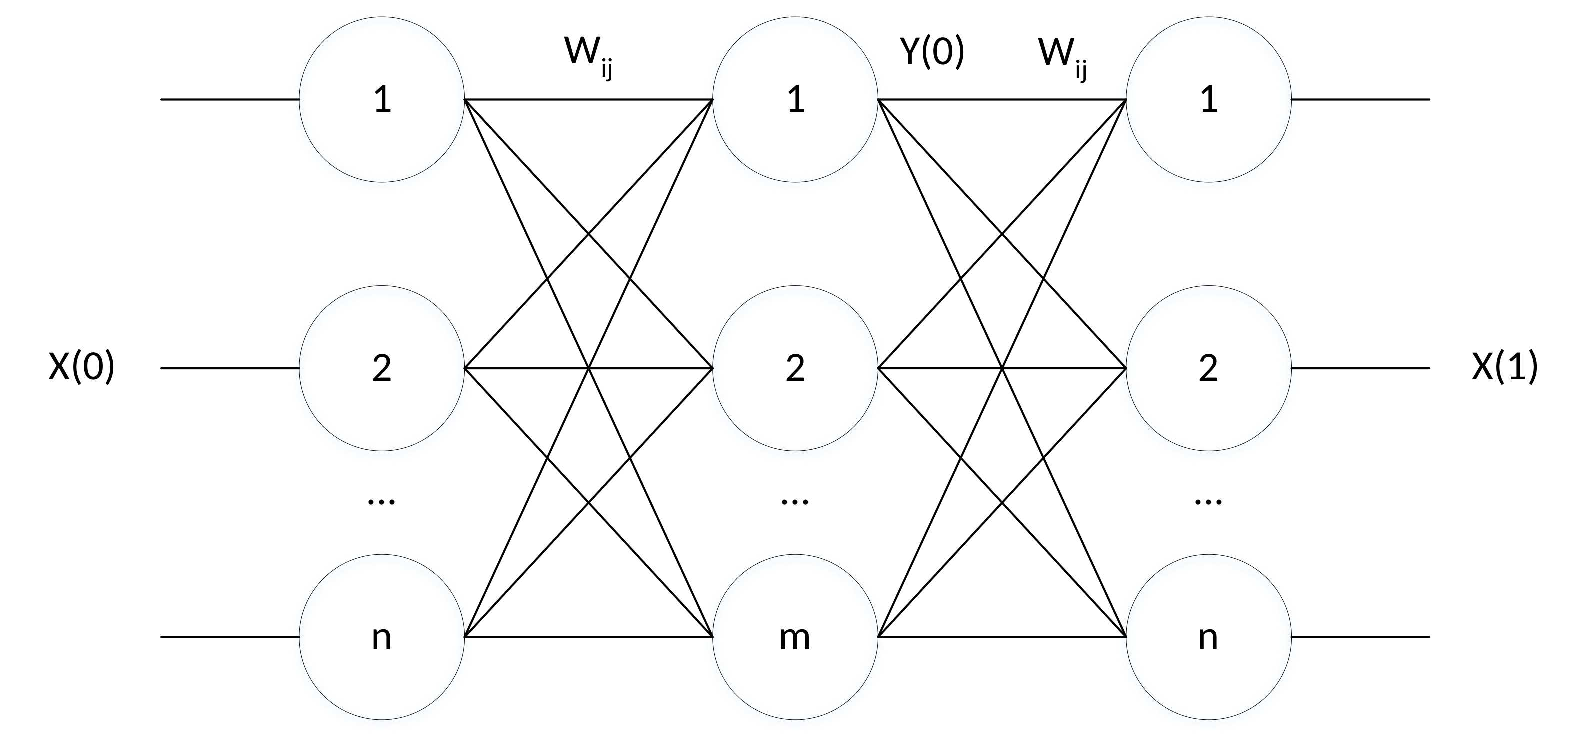
\includegraphics[width=0.9\textwidth]{man-source/images/ch2/pic2-1.pdf}
  \caption{Развернутое представление RBM}
  \label{fig:pic2_1}
\end{figure}

Представим сэмплирование Гиббса, используя развернутое представление RBM (рисунок~\ref{fig:pic2_2}).

\begin{figure}[H]
  \centering
  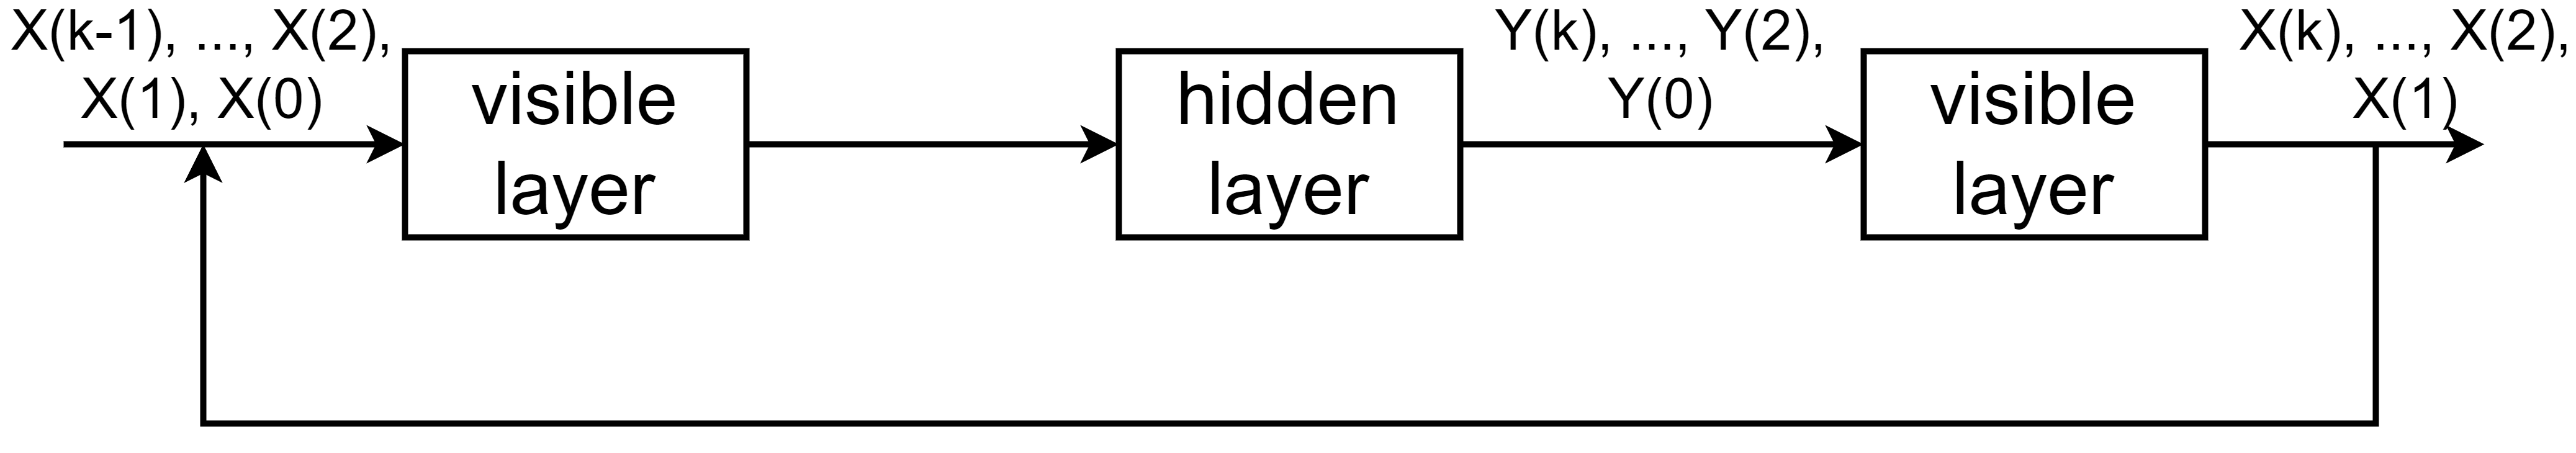
\includegraphics[width=\textwidth]{man-source/images/ch2/pic2-2.png}
  \caption{Сэмплирование Гиббса}
  \label{fig:pic2_2}
\end{figure}

Сэмплирование Гиббса заключается в следующей процедуре. Пусть $x(0)$ -- входной вектор, который поступает на видимый слой в момент времени $t=0$. Тогда выходные значения нейронов скрытого слоя будут определяться следующим образом:

\begin{equation}
    y_j(0)=F(S_j(0)),
\end{equation}

\begin{equation}
    S_j(0)=\sum_i w_{ij}x_i(0)+T_j.
\end{equation}

Инверсный (последний) слой  реконструирует входной вектор на основе данных со скрытого слоя и текущего значения настраиваемых параметров (порогов видимого слоя и матрицы весов). В результате получается восстановленный вектор $x(1)$ в момент времени $t=1$:

\begin{equation}
    x_i(1)=F(S_i(1)),
\end{equation}

\begin{equation}
    S_i(1)=\sum_j w_{ij}y_j(0)+T_i.
\end{equation}

Затем вектор $x(1)$ поступает на видимый слой, и вычисляются выходные значения нейронов скрытого слоя: 

\begin{equation}
    y_j(1)=F(S_j(1)),
\end{equation}

\begin{equation}
    S_j(1)=\sum_i w_{ij}x_i(1)+T_j.
\end{equation}

Продолжая данный процесс, можно получить на шаге k следующие выражения:

\begin{equation*}		
    y_j(k)=F(S_j(k)),\ S_j(k)=\sum_i w_{ij}x_i(k)+T_j.
\end{equation*}

\begin{equation*}		
    x_i(k)=F(S_i(k)),\ S_i(k)=\sum_j w_{ij}y_j(k-1)+T_i.
\end{equation*}

\section{Вывод правил предобучения} 

Хинтоном была предложена энергетическая модель, базирующаяся на идее максимизации функции правдоподобия распределения входных данных $P(x)$. Вывод классических правил обучения был приведен в главе I. Основываясь на идее использования ограниченной машины Больцмана в качестве вспомогательной модели для проведения предобучения, было предложено использование двух разных критериев для ее обучения \cite{4-A}. Первый критерий основывается на минимизации среднеквадратичной ошибки (MSE), а второй -- на минимизации кросс-энтропийной функции ошибки.

Покажем, что применение различных критериев минимизации позволяет, тем не менее, получить одинаковые правила обучения.

\subsection{Критерий MSE}

В случае использования в качестве критерия обучения MSE основной целью обучения ограниченной машины Больцмана является минимизация суммарной среднеквадратичной ошибки реконструкции данных на скрытом и видимом (восстанавливающем) слое, которая в случае CD-k определяется следующим образом:	

\begin{equation*}	
    E_s(k)=\frac{1}{2L}\Bigg(\sum_{l=1}^L\sum_{j=1}^m\sum_{p=1}^k (y_j^l(p)-y_j^l(p-1))^2+\sum_{l=1}^L\sum_{i=1}^n\sum_{p=1}^k (x_i^l(p)-x_i^l(p-1))^2\Bigg)
\end{equation*}
где \textit{k} определяет параметр процедуры сэмплирования Гиббса, \textit{n} -- количество нейронов в видимом слое, \textit{m} -- количество нейронов в скрытом слое, \textit{L} -- размерность обучающей выборки.

В случае CD-1  суммарная среднеквадратичная ошибка	

\begin{equation}
    E_s(1)=\frac{1}{2L}\Bigg(\sum_{l=1}^L\sum_{j=1}^m (y_j^l(1)-y_j^l(0))^2+\sum_{l=1}^L\sum_{i=1}^n (x_i^l(1)-x_i^l(0))^2\Bigg)
\end{equation}

Как следует из приведенных выше выражений ошибка состоит из двух частей: ошибки восстановления информации на видимом и скрытом слоях, т.е. может быть представлена в следующем виде:
\begin{equation}
	\label{mse_rbm_criteria}
	E_s(k) = E_h(k) + E_v(k)
\end{equation}
где

\begin{equation}
	E_h(k) = \frac{1}{2L}\sum_{l=1}^L\sum_{j=1}^m\sum_{p=1}^k (y_j^l(p)-y_j^l(p-1))^2
\end{equation}

\begin{equation}
	E_v(k) = \frac{1}{2L}\sum_{l=1}^L\sum_{i=1}^n\sum_{p=1}^k (x_i^l(p)-x_i^l(p-1))^2
\end{equation}

Найдем правила обучения, соответствующие критерию \ref{mse_rbm_criteria} и докажем их эквивалентность классическим правилам обучения RBM при выполнении некоторых специальных условий.

\textbf{Теорема 1}. Максимизация функции правдоподобия распределения данных $P(x)$ в пространстве синаптических связей ограниченной машины Больцмана эквивалентна минимизации суммарной квадратичной ошибки сети в том же пространстве при использовании линейных нейронов.

\textbf{Доказательство}: Рассмотрим последовательное обучение RBM, когда модификация синаптических связей происходит после подачи каждого входного образа на сеть (онлайн-обучение). В соответствии с методом градиентного спуска для минимизации суммарной квадратичной ошибки сети, синаптические связи должны изменяться следующим образом:	

\begin{equation}
w_{ij}(t+1)=w_{ij}(t)-\alpha\frac{\partial E}{\partial w_{ij}(t)},
\end{equation}		

\begin{equation}
T_{i}(t+1)=T_{i}(t)-\alpha\frac{\partial E}{\partial T_{i}(t)},
\end{equation}		

\begin{equation}
T_{j}(t+1)=T_{j}(t)-\alpha\frac{\partial E}{\partial T_{j}(t)},
\end{equation}

В случае CD-k квадратичная ошибка $E$ для одного образа:

\begin{equation*}
E=\frac{1}{2}\sum_{j=1}^m\sum_{p=1}^k (y_j(p)-y_j(p-1))^2+\frac{1}{2}\sum_{i=1}^n\sum_{p=1}^k (x_i(p)-x_i(p-1))^2
\end{equation*}

Тогда
\begin{multline*}
    \frac{\partial E}{\partial w_{ij}}=\frac{\partial E}{\partial y_j(p)}\frac{\partial y_j(p)}{\partial S_j(p)}\frac{\partial S_j(p)}{\partial w_{ij}}+\frac{\partial E}{\partial x_i(p)}\frac{\partial x_i(p)}{\partial S_i(p)}\frac{\partial S_i(p)}{\partial w_{ij}}=\\=\sum_{p=1}^k (y_j(p)-y_j(p-1))x_i(p)F'(S_j(p))+\\+\sum_{p=1}^k (x_i(p)-x_i(p-1))y_j(p-1)F'(S_i(p))
\end{multline*}

Если ограниченная машина Больцмана использует линейные нейроны с линейной функцией активации, то

\begin{equation*}
    \frac{\partial S_i(p)}{\partial w_{ij}}=F'(S_i(p))=\frac{\partial S_j(p)}{\partial w_{ij}}=F'(S_j(p))=1,
\end{equation*}

Тогда

\begin{equation*}
    \frac{\partial E}{\partial w_{ij}}=\sum_{p=1}^k (y_j(p)x_i(p)-y_j(p-1)x_i(p-1))=y_j(k)x_i(k)-y_j(0)x_i(0),
\end{equation*}

В результате можно получить CD-k правило обучения RBM:

\begin{equation*}
    w_{ij}(t+1)=w_{ij}(t)+\alpha(x_i(0)y_j(0)-x_i(k)y_j(k)),
\end{equation*}

Аналогичным образом для пороговых значений:

\begin{equation*}
\begin{aligned}
    T_{j}(t+1)=T_{j}(t)+\alpha(y_j(0)-y_j(k)),\\
    T_{i}(t+1)=T_{i}(t)+\alpha(x_i(0)-x_i(k))
\end{aligned}
\end{equation*}

Как видно последние выражения совпадают с классическим правилом обучения ограниченной машины Больцмана для CD-k. Отсюда следует, что для линейной RBM максимизация функции правдоподобия распределения данных $P(x)$ эквивалентна минимизации суммарной квадратичной ошибки сети. Теорема доказана.

\textbf{Следствие 1.1}. Линейная ограниченная машина Больцмана c точки зрения обучения эквивалентна автоассоциативной нейронной сети при использовании в ней при обучении сэмплирования Гиббса.

\textbf{Следствие 1.2}. Для нелинейной ограниченной машины Больцмана правило модификации синаптических связей в случае CD-k будет следующим:
\begin{multline*}
    w_{ij}(t+1)=w_{ij}(t)-\\-\alpha\Bigg(\sum_{p=1}^k (y_j(p)-y_j(p-1))x_i(p)F'(S_j(p))+(x_i(p)-x_i(p-1))y_j(p-1)F'(S_i(p))\Bigg)
\end{multline*}

\begin{equation*}
\begin{aligned}
    T_i(t+1)=T_i(t)-\alpha\left(\sum_{p=1}^k (x_i(p)-x_i(p-1))F'(S_i(p))\right),\\
    T_j(t+1)=T_j(t)-\alpha\left(\sum_{p=1}^k (y_j(p)-y_j(p-1))F'(S_j(p))\right),
\end{aligned}
\end{equation*}

\textbf{Следствие 1.3}. Для нелинейной ограниченной машины Больцмана правило модификации синаптических связей в случае CD-1 будет следующим:	
\begin{equation*}
    w_{ij}(t+1)=w_{ij}(t)-\alpha((y_j(1)-y_j(0))F'(S_j(1))x_i(1)+(x_i(1)-x_i(0))F'(S_i(1))y_j(0)),
\end{equation*}

\begin{equation*}
    T_i(t+1)=T_i(t)-\alpha(x_i(1)-x_i(0))F'(S_i(1)),
\end{equation*}

\begin{equation*}
    T_j(t+1)=T_j(t)-\alpha(y_j(1)-y_j(0))F'(S_j(1)).  
\end{equation*}

При использовании группового обучения (batch learning), метод градиентного спуска примет следующий вид:

\begin{equation}
    w_{ij}(t+1)=w_{ij}(t)-\alpha\frac{\partial E_s}{\partial w_{ij}(t)}
\end{equation}

\begin{equation}
    T_{i}(t+1)=T_{i}(t)-\alpha\frac{\partial E_s}{\partial T_{i}(t)}
\end{equation}

\begin{equation}
    T_{j}(t+1)=T_{j}(t)-\alpha\frac{\partial E_s}{\partial T_{j}(t)}.
\end{equation}

\textbf{Теорема 2}. При использовании  CD-k для нелинейной ограниченной машины Больцмана в случае группового обучения правило модификации синаптических связей определяется на основе следующих выражений:
\begin{multline*}
    w_{ij}(t+1)=w_{ij}(t)-\\-\frac{\alpha}{L}\Bigg(\sum_{l=1}^L\sum_{p=1}^k (y_j^l(p)-y_j^l(p-1))x_i^l(p)F'(S_j^l(p))+(x_i^l(p)-x_i^l(p-1))y_j^l(p-1)F'(S_i^l(p))\Bigg),
\end{multline*}

\begin{equation*}
    T_{i}(t+1)=T_{i}(t)-\frac{\alpha}{L}\left(\sum_{l=1}^L\sum_{p=1}^k (x_i^l(p)-x_i^l(p-1))F'(S_i^l(p))\right),
\end{equation*}

\begin{equation*}
    T_{j}(t+1)=T_{j}(t)-\frac{\alpha}{L}\left(\sum_{l=1}^L\sum_{p=1}^k (y_j^l(p)-y_j^l(p-1))F'(S_j^l(p))\right)
\end{equation*}

Процесс доказательства данной теоремы является аналогичным доказательству теоремы 1.

\textbf{Следствие 2.1}. При использовании  CD-1 для нелинейной ограниченной машины Больцмана в случае группового обучения правило модификации синаптических связей определяется на основе следующих выражений:

\begin{multline*}
    w_{ij}(t+1)=w_{ij}(t)-\\-\frac{\alpha}{L}\left(\sum_{l=1}^L (y_j^l(1)-y_j^l(0))x_i^l(1)F'(S_j^l(1))+(x_i^l(1)-x_i^l(0))y_j^l(0)F'(S_i^l(1))\Bigg)\right.,
\end{multline*}

\begin{equation*}
    T_i(t+1)=T_i(t)-\frac{\alpha}{L}\left(\sum_{l=1}^L (x_i^l(1)-x_i^l(0))F'(S_i^l(1))\right),
\end{equation*}

\begin{equation*}
    T_j(t+1)=T_j(t)-\frac{\alpha}{L}\left(\sum_{l=1}^L (y_j^l(1)-y_j^l(0))F'(S_j^l(1))\right)
\end{equation*}

\textbf{Следствие 2.2}. При использовании  CD-k для линейной ограниченной машины Больцмана в случае группового обучения правило модификации синаптических связей определяется на основе следующих выражений:

\begin{equation*}
    w_{ij}(t+1)=w_{ij}(t)+\frac{\alpha}{L}\sum_{l=1}^L (x_i^l(0)y_j^l(0)-x_i^l(k)y_j^l(k)),
\end{equation*}

\begin{equation*}
    T_{i}(t+1)=T_{i}(t)+\frac{\alpha}{L}\sum_{l=1}^L (x_i^l(0)-x_i^l(k)),
\end{equation*}

\begin{equation*}
    T_{j}(t+1)=T_{j}(t)+\frac{\alpha}{L}\sum_{l=1}^L (y_j^l(0)-y_j^l(k))
\end{equation*}

\textbf{Следствие 2.3}. При использовании  CD-1 для линейной ограниченной машины Больцмана в случае группового обучения правило модификации синаптических связей определяется на основе следующих выражений:

\begin{equation*}
    w_{ij}(t+1)=w_{ij}(t)+\frac{\alpha}{L}\sum_{l=1}^L (x_i^l(0)y_j^l(0)-x_i^l(1)y_j^l(1)),
\end{equation*}

\begin{equation*}
    T_{i}(t+1)=T_{i}(t)+\frac{\alpha}{L}\sum_{l=1}^L (x_i^l(0)-x_i^l(1)),
\end{equation*}

\begin{equation*}
    T_{j}(t+1)=T_{j}(t)+\frac{\alpha}{L}\sum_{l=1}^L (y_j^l(0)-y_j^l(1))
\end{equation*}

Таким образом, получены правила обучения для ограниченной машины Больцмана, которые базируются на минимизации квадратичной ошибки восстановления информации на видимом и скрытом слоях.  Предложенный метод позволяет учитывать нелинейную природу нейронных элементов. Показано, что классические выражения для обучения ограниченной машины являются частным случаем предложенного метода. Доказана теорема об эквивалентности максимизации функции правдоподобия распределения входных данных $P(x)$ и минимизации суммарной квадратичной ошибки сети в одном и том же пространстве синаптических связей для линейной ограниченной машины Больцмана. 

% Впервые подход был представлен в \cite{n9} для случая CD-1 и в \cite{Golovko2015a, Golovko2015b} для случая CD-k.

\subsection{Критерий СЕ}

В случае CD-k кросс-энтропийная функция ошибки для видимого слоя определяется следующим образом:

\begin{equation*}
	CE_v(k) = -\frac{1}{L}\sum_{l=1}^L \sum_{p=1}^k \sum_{i=1}^n x_i^l(p-1)\log(x_i^l(p))+(1-x_i^l(p-1)\log(1-x_i^l(p))
\end{equation*}
где $L$ -- размер обучающей выборки, $k$ -- параметр процедуры сэмплирования, $n$ -- количество нейронов на видимом слое.

Аналогично для скрытого слоя:

\begin{equation*}
	CE_h(k) = -\frac{1}{L}\sum_{l=1}^L \sum_{p=1}^k \sum_{j=1}^m y_j^l(p-1)\log(y_j^l(p))+(1-y_j^l(p-1)\log(1-y_j^l(p))
\end{equation*}
где $m$ -- количество нейронов на скрытом слое.

Общая функция определяется как сумма кросс-энтропийных функций ошибки видимого и скрытого слоев:

\begin{equation}
	CE_s(k) = CE_h(k)+CE_v(k)
\end{equation}

Докажем следующую теорему.

\textbf{Теорема 3}. Максимизация функции правдоподобия распределения входных данных $P(x)$ эквивалентна минимизации кросс-энтропийной целевой функции $CE_s(k)$ в одном и том же пространстве синаптических весов ограниченной машины Больцмана (случай $k=1$).

\textbf{Доказательство}. В случае CD-1 кросс-энтропийная функция для одного обучающего примера будет иметь следующий вид:

\begin{multline}
	CE(1) = -\sum_{i=1}^n (x_i(0)\log(x_i(1))+(1-x_i(0))\log(1-x_i(1)))-\\-\sum_{j=1}^m ( y_j(0)\log(y_j(1))+(1-y_j(0))\log(1-y_j(1))) = CE_v(1)+CE_h(1)
\end{multline}

Найдем частные производные кросс-энтропийной функции по весовым элементам. Получим

\begin{equation*}
	\frac{\partial CE(1)}{\partial w_{ij}} = \frac{\partial CE_v(1)}{\partial w_{ij}} + \frac{\partial CE_h(1)}{\partial w_{ij}}
\end{equation*}

Тогда

\begin{multline*}
	\frac{\partial CE_v(1)}{\partial w_{ij}} = -\frac{x_i(0)}{x_i(1)}x_i(1)(1-x_i(1))y_j(0)+\frac{1-x_i(0)}{1-x_i(1)}x_i(1)(1-x_i(1))y_j(0) = \\ = -x_i(0)(1-x_i(1))y_j(0)+(1-x_i(0))x_i(1)y_j(0)=\\=-x_i(0)y_j(0)+x_i(0)x_i(1)y_j(0)+x_i(1)y_j(0)-x_i(0)x_i(1)y_j(0)=\\=-x_i(0)y_j(0)+x_i(1)y_j(0) 
\end{multline*}

и

\begin{multline*}
	\frac{\partial CE_h(1)}{\partial w_{ij}} = -y_j(0)(1-y_j(1))x_i(1)+(1-y_j(0))y_j(1)x_i(1) = \\ = -y_j(0)x_i(0)+y_j(0)y_j(1)x_i(1)+y_j(1)x_i(1)-y_j(0)y_j(1)x_i(1) = \\ = -y_j(0)x_i(1)+y_j(1)x_i(1). 
\end{multline*}

Окончательно получим

\begin{multline*}
	\frac{\partial CE(1)}{\partial w_{ij}} = \frac{\partial CE_v(1)}{\partial w_{ij}} + \frac{\partial CE_h(1)}{\partial w_{ij}} = \\ = -x_i(0)y_j(0)+x_i(1)y_j(0) -y_j(0)x_i(1)+y_j(1)x_i(1) = x_i(1)y_j(1) - x_i(0)y_j(0).
\end{multline*}

Аналогично, для пороговых элементов имеем:

\begin{multline*}
	\frac{\partial CE(1)}{\partial T_i} = \frac{\partial CE_v(1)}{\partial T_i} = -\frac{x_i(0)}{x_i(1)}x_i(1)(1-x_i(1))+\frac{1-x_i(0)}{1-x_i(1)}x_i(1)(1-x_i(1)) = \\ = -x_i(0) + x_i(0)x_i(1)+x_i(1)-x_i(0)x_i(1) = x_i(1)-x_i(0) 
\end{multline*}

\begin{multline*}
	\frac{\partial CE(1)}{\partial T_j} = \frac{\partial CE_h(1)}{\partial T_j} = -y_j(0)(1-y_j(1)) + (1-y_j(0))y_j(1) = \\ = -y_j(0) + y_j(0)y_j(1) + y_j(1) - y_j(0)y_j(1) = y_j(1) - y_j(0).
\end{multline*}

Теорема доказана. 

Рассматривая более общий случай CD-k, можно доказать следующую теорему.

\textbf{Теорема 4}. Максимизация функции правдоподобия распределения входных данных $P(x)$ эквивалентна минимизации кросс-энтропийной целевой функции $CE_s(k)$ в одном и том же пространстве синаптических весов ограниченной машины Больцмана (случай произвольного $k$).

\textbf{Доказательство}. В случае CD-k кросс-энтропийная функция для одного обучающего примера будет иметь следующий вид:

\begin{multline}
	CE_s(k) = -\sum_{p=1}^k \sum_{i=1}^n (x_i(p-1)\log(x_i(p)) + (1-x_i(p-1))\log(1-x_i(p)))-\\-\sum_{p=1}^k \sum_{j=1}^m (y_j(p-1)\log (y_j(p))+(1-y_j(p-1))\log(1-y_j(p))) = CE_v(k) + CE_h(k)
\end{multline}

Как и в случае CD-1 находим соответствующие частные производные по весовым и пороговым элементам. Имеем:

\begin{equation*}
	\frac{\partial CE_s(k)}{\partial w_{ij}}= \frac{\partial CE_v(k)}{\partial w_{ij}} + \frac{\partial CE_h(k)}{\partial w_{ij}}
\end{equation*}

Причем

\begin{multline*}
	\frac{\partial CE_v(k)}{\partial w_{ij}} = \\ = -\sum_{p=1}^k (x_i(p-1)(1-x_i(p))y_j(p-1)-(1-x_i(p-1))x_i(p)y_j(p-1))=\\=-\sum_{p=1}^k (x_i(p-1)y_j(p-1)-x_i(p-1)x_i(p)y_j(p-1)-\\-x_i(p)y_j(p-1)+x_i(p-1)x_i(p)y_j(p-1)) = \\ = \sum_{p=1}^{k} (x_i(p)y_j(p-1)-x_i(p-1)y_j(p-1))
\end{multline*}

и

\begin{multline*}
	\frac{\partial CE_h(k)}{\partial w_{ij}} = \\ = -\sum_{p=1}^k (y_j(p-1)(1-y_j(p))x_i(p)-(1-y_j(p-1))y_j(p)x_i(p)) = \\ = -\sum_{p=1}^{k} (y_j(p-1)x_i(p)-y_j(p-1)y_j(p)x_i(p)-\\-y_j(p)x_i(p)+y_j(p-1)y_j(p)x_i(p)) = \\ = \sum_{p=1}^{k} (x_i(p)y_j(p)-x_i(p)y_j(p-1)).
\end{multline*}

А значит

\begin{multline*}
	\frac{\partial CE_s(k)}{\partial w_{ij}} = \sum_{p=1}^{k}(y_j(p)x_i(p)-x_i(p-1)y_j(p-1)) = \\ = y_j(1)x_i(1)-x_i(0)y_j(0)+x_i(2)y_j(2)-x_i(1)y_j(1)+\dots+\\+x_i(k)y_j(k)-x_i(k-1)y_j(k-1)=\\=x_i(k)y_j(k)-x_i(0)y_j(0).
\end{multline*}

Аналогично для пороговых элементов:

\begin{multline*}
	\frac{\partial CE_s(k)}{\partial T_i} = \frac{\partial CE_v(k)}{\partial T_i} =\\= -\sum_{p=1}^k (x_i(p-1)(1-x_i(p))-(1-x_i(p-1))x_i(p)) =\\= \sum_{p=1}^k (x_i(p) - x_i(p-1)) = x_i(1)-x_i(0)+x_i(2) - x_i(1) +\dots+x_i(k)-x_i(k-1) =\\= x_i(k)-x_i(0).
\end{multline*}

\begin{multline*}
	\frac{\partial CE_s(k)}{\partial T_j} = \frac{\partial CE_h(k)}{\partial T_j} =\\= -\sum_{p=1}^k (y_j(p-1)(1-y_j(p))-(1-y_j(p-1))y_j(p)) =\\= \sum_{p=1}^k (y_j(p) - y_j(p-1)) = y_j(1)-y_j(0)+y_j(2) - y_j(1) +\dots+y_j(k)-y_j(k-1) =\\= y_j(k)-y_j(0).
\end{multline*}

Теорема доказана.

Из доказанных теорем 3 и 4 следует, что правила обучения ограниченной машины Больцмана могут быть получены более простым путем, чем при использовании традиционного подхода, основанного на применении функции энергии. Произведя минимизацию кросс-энтропийной функции и применяя простые итерации сэмплирования Гиббса, мы получили классические линейные правила обучения RBM.

Таким образом, на основании доказанных теорем 1-4 можно сформулировать общую теорему.

\textbf{Теорема 5}. Максимизация функции правдоподобия распределения входных данных $P(x)$ эквивалентна минимизации кросс-энтропийной функции и специальному случаю минимизации среднеквадратичной ошибки в одном и том же пространстве синаптических весов ограниченной машины Больцмана:

\begin{equation}
	\max(\ln P(x)) = \min(CE_s) = \min(E_s)
\end{equation}

Теорема 5 обобщает предыдущие результаты. Как следует из этой теоремы, использование различных критериев обучения приводит к тем же самым правилам. Поэтому сущность неконтролируемого обучения для ограниченной машины Больцмана одинакова, даже если используются различные целевые функции. Максимизация функции правдоподобия и минимизация кросс-энтропийной функции ошибки приводит к линейному представлению нейронных элементов в терминах минимизации функции MSE. Необходимо отметить, что, применяя критерий MSE, мы учитываем также нелинейное представление нейронных элементов. Таким образом, очевидное преимущество в использовании MSE в качестве функции ошибок перед применением функции максимального правдоподобия и кросс-энтропийной функции в том, что при использовании MSE могут быть получены как линейные, так и нелинейные правила обучения.

В дальнейшем для идентификации предлагаемого подхода будем использовать аббревиатуру REBA (Reconstruction Error-Based Approach). Классический метод будем называть C-RBM (Classic Restricted Boltzmann Machine Training).

\section{Предобучение сверточных слоев}

Выполнение предобучения сверточных слоев имеет особое значение при решении задач компьютерного зрения в силу эффективности таких слоев при обработке визуальной информации, представленной с помощью отдельных изображений и видео.

Отметим, что преобразования, выполняемые над сверточными слоями при обучении, идентичны преобразованиям для полносвязных слоев. 
Отличие заключается в операции <<развертки>> (deconvolution), которая используется на этапе предобучения при реконструкции активности видимых нейронов и на этапе тонкой настройки для метода обратного распространения при вычислении ошибок на скрытых слоях сети. Эта операция применяется в сверточных нейронных сетях для повышения частоты дискретизации.
Рассмотрим визуальное представление операции свертки для случая карт 3Х3 и 2Х2 (рис. \ref{fig:convolution}).

\begin{figure}[H]
  \centering
  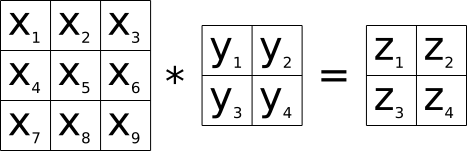
\includegraphics[width=0.5\textwidth]{man-source/images/ch2/pic2-4.png}
  \caption{Операция свертки}
  \label{fig:convolution}
\end{figure}

Сверточный слой с одним ядром может быть представлен в виде разряженного слоя, а операция <<развертки>> -- слоем, полученным применением симметричного преобразования относительно разряженного. При этом полученная сеть представляет собой автоэнкодер с симметричными связями относительно скрытого слоя (рис. \ref{fig:convolution_autoencoder}).

На основании данного представления могут быть получены формулы для выполнения <<развертки>>:

\begin{equation*}
	x'_1 = z_1y_1		
	\end{equation*}
	\begin{equation*}
	x'_2 = z_1y_2+z_2y_1
	\end{equation*}
	\begin{equation*}
	x'_3 = z_2y_2
	\end{equation*}
	\begin{equation*}
	x'_4 = z_1y_3 + z_3y_1
	\end{equation*}
	\begin{equation*}
	x'_5 = z_1y_4 + z_2y_3 + z_3y_2 + z_4y_1
	\end{equation*}
	\begin{equation*}
	x'_6 = z_2y_4 + z_4y_2
	\end{equation*}
	\begin{equation*}
	x'_7 = z_3y_3
	\end{equation*}
	\begin{equation*}
	x'_8 = z_3y_4 + z_4y_3
	\end{equation*}		
	\begin{equation*}
	x'_9 = z_4y_4
	\end{equation*}	

Сама операция <<развертки>> представлена на рис. \ref{fig:deconvolution}.

\begin{figure}[H]
  \centering
  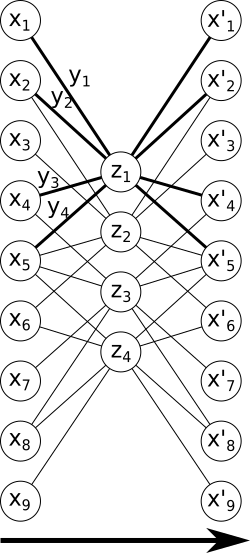
\includegraphics[width=0.4\textwidth]{man-source/images/ch2/pic2-5.png}
  \caption{Разряженный автоэнкодер операции свертки}
  \label{fig:convolution_autoencoder}
\end{figure}

\begin{figure}[H]
  \centering
  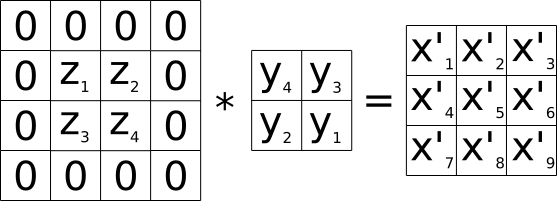
\includegraphics[width=0.6\textwidth]{man-source/images/ch2/pic2-6.png}
  \caption{Операция <<развертки>>}
  \label{fig:deconvolution}
\end{figure}

Введя операции матричного поворота на 180 градусов и заполнения нулями границ матрицы (padding), можно получить следующие общие формулы для выполнения <<развертки>> (рис. \ref{fig:deconvolution_formula}).

\begin{figure}[H]
  \centering
  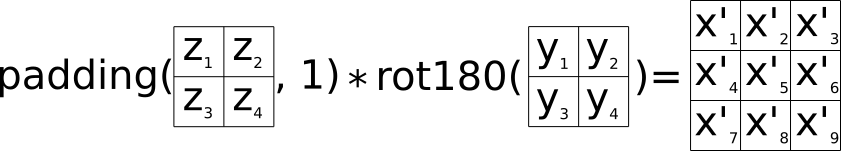
\includegraphics[width=0.9\textwidth]{man-source/images/ch2/pic2-9.png}
  \caption{Формула <<развертки>>}
  \label{fig:deconvolution_formula}
\end{figure}

Введем условное обозначение для операции <<развертки>> -- $\circledast$.

Применяя полученную формулу для выполнения <<развертки>>, можно осуществлять процедуру CD на сверточных слоях ГНС, которые в этом случае рассматриваются как сверточные ограниченные машины Больцмана (CRBM). 

Рассмотрим формулы для получения необходимых карт признаков для расчета градиента изменения параметров слоя в случае использования процедуры CD-1: 

\begin{equation*}
    y_j(0) = F(x_i(0) * w_{ij} + T_j)
\end{equation*}

\begin{equation*}
    x_i(1) = F(y_j(0) \circledast w_{ij} + T_i)
\end{equation*}

\begin{equation*}
    y_j(1) = F(x_i(1) * w_{ij} + T_j)
\end{equation*}
где $w_{ij}$ -- $i$-тый компонент $j$-того ядра свертки, $x_i(0)$ -- $i$-тый компонент входной карты признаков, $T_j$ -- пороговый элемент $j$-того нейрона скрытого слоя, $y_j(0)$ -- $j$-тый компонент выходной карты признаков, $x_i(1)$ -- $i$-тый компонент реконструированной входной карты признаков, $T_i$ -- пороговый элемент $i$-того нейрона видимого слоя, $y_j(1)$ -- $j$-тый компонент реконструированной выходной карты признаков.

Классические правила обучения RBM могут быть переформулированы для случая CRBM (CD-1, последовательное обучение): 

\begin{equation*}
		w_{ij}(t+1)=w_{ij}(t)+\alpha(x_i(0) * y_j(0)-x_i(1) * y_j(1))
\end{equation*} 

\begin{equation*}	
		T_i(t+1)=T_i(t)+\alpha(x_i(0)-x_i(1))
\end{equation*} 

\begin{equation*}		
		T_j(t+1)=T_j(t)+\alpha(y_j(0)-y_j(1))
\end{equation*}
% где $\circledast$ обозначает операцию свертки.

В соответствии с предлагаемым методом, правила обучения могут быть переформулированы следующим образом (CD-1, последовательное обучение):

\begin{multline*}
    w_{ij}(t+1)=w_{ij}(t)-\alpha((y_j(1)-y_j(0))F'(S_j(1)) * x_i(1)+\\(x_i(1)-x_i(0))F'(S_i(1)) * y_j(0)),    
\end{multline*}
\begin{equation*}
    T_i(t+1)=T_i(t)-\alpha(x_i(1)-x_i(0))F'(S_i(1)),
\end{equation*}
\begin{equation*}
    T_j(t+1)=T_j(t)-\alpha(y_j(1)-y_j(0))F'(S_j(1)).  
\end{equation*}

Аналогичным образом могут быть получены правила для CD-\textit{k} случая процедуры обучения и группового случая.

Таким образом, для глубокой сверточной нейронной сети, содержащей слои разных типов (полносвязные и сверточные) возможно сочетание нескольких вариантов обучения -- с представлением в виде CRBM (для сверточных слоев) и в виде RBM (для полносвязных).  

\section{Метод редуцирования параметров}
Известно, что полносвязные нейронные сети обладают определенной степенью избыточности. Полносвязный слой в сравнении со сверточным содержит большее количество настраиваемых параметров, однако в задачах компьютерного зрения сверточные нейронные сети показывают существенно лучшие результаты по обобщающей способности, чем полносвязные. Таким образом, очевидно, что в полносвязных сетях при большем количестве настраиваемых параметров, они используются менее оптимально. Можно предположить, что указанные <<избыточные>> параметры могут быть исключены без существенного ухудшения эффективности работы модели. Важный вопрос, возникающий при выполнении такой операции редуцирования, касается самого алгоритма отсеивания малоинформативных параметров.

К основным методам компрессии (сжатия) нейросетевых моделей на настоящий момент относятся:
\begin{easylistNum}
	& прунинг -- pruning (\cite{wang2019pruning}, \cite{xu2020});
	& квантизация -- quantization \cite{hubara2016quantized};
	& дистилляция -- distillation \cite{Hinton2015DistillingTK};
	& матричная факторизация низкого ранга -- low-rank matrix factorization \cite{Sainath2013}.
\end{easylistNum}

\textit{Прунинг} позволяет удалить часть связей и нейронов (в зависимости от выполняемой техники редуцирования), что уменьшает структурную избыточность <<тяжелых>> глубоких нейросетевых моделей.
По типу выполняемой техники прунинга выделяют:

\begin{easylist}
	& прунинг связей;
	& прунинг нейронов или фильтров (в зависимости от типа слоя -- полносвязного или сверточного);
	& прунинг слоев.
\end{easylist}

\textit{Квантизация} используется для физического уменьшения памяти, занимаемой моделью. В этом подходе осуществляется редуцирование типа данных, используемого для хранения параметров нейросетевой модели (например, осуществляется переход от 32-битного к 16-битному или 8-битному представлению типа).

\textit{Дистилляция} основывается на возможности использования более <<тяжелых>> моделей для обучения моделей меньшего размера. В этом случае обученная модель-учитель генерирует примеры, которые используются для обучения модели-ученика. Размер такой модели-ученика может быть существенно меньше первоначальной сети. По разновидностям выделяют следующие типы дистилляции:

\begin{easylist}
	& офлайн-дистилляция (применяется последовательное обучение модели-учителя, затем -- модели-ученика);
	& онлайн-дистилляция (применяется одновременное обучение модели-учителя и модели-ученика);
	& самодистилляция (в качестве модели-учителя и модели-ученика выступает одна модель).
\end{easylist}

Наконец, \textit{матричная факторизация низкого ранга} позволяет осуществить декомпозицию матрицы весовых коэффициентов большого размера на совокупность матриц меньшего размера. Применение данного подхода помогает уменьшить память, занимаемую моделями и ускорить время работы модели. К недостаткам метода относят его вычислительную сложность.
% Редуцирование параметров нейросетевой модели позволяет добиться уменьшения количества настраиваемых параметров, что может быть актуальным при применении нейронных сетей на устройствах с ограниченными аппаратными возможностями (одноплатные компьютеры, мобильные телефоны и т.д.). Применение при этом специальных методик для хранения разряженных матриц позволяет ускорить работу архитектуры. Важно, чтобы при этом сеть сохраняла свою обобщающую способность.

Предлагаемый алгоритм редуцирования связей НС основывается на прунинге, но имеет модификацию, которая заключается в наличии этапа неконтролируемого предобучения на основе RBM.

Рассмотрим подход для редуцирования связей полносвязной нейронной сети, основанный на использовании предобучения. Первый и четвертый этапы данной процедуры аналогичны этапам выполнения предобучения типа II, описанного в главе I. В ходе выполнения дополнительных этапов 2 и 3 формируются разряженные связи между входными и выходными нейронными элементами слоя и уменьшается его размерность за счет удаления части нейронных элементов, которые не используются при <<тонкой настройке>> и дальнейшей эксплуатации нейросетевой модели (рисунок~\ref{fig:pic2_3}):
\begin{easylistNum}
    & Неконтролируемое предобучение НС с использованием <<жадного>> алгоритма, начиная с первого слоя. Параметры каждого слоя, представленные весовыми и пороговыми коэффициентами, настраиваются в соответствии с правилами обучения ограниченной машины Больцмана;
    & <<Обнуление>> весовых коэффициентов слоев нейронной сети, абсолютные значения которых не превышают некоторый заданный порог $t > 0$. Иначе говоря, параметры со значениями, попадающими в интервал $[-t, t]$, не изменяются при дальнейшем обучении;
    & Архитектурная реконфигурация нейронной сети, в ходе которой удаляются нейроны, не участвующие в формировании выходной активности сети (нейроны, имеющие нулевые векторы весовых коэффициентов или, в случае использования сверточных слоев, нейроны, имеющие нулевые ядра свертки). Реконфигурация выполняется в соответствии со следующими правилами:\\
        для каждого \textit{i}-того слоя НС, кроме первого и последнего:
        \begin{itemize}
            \item если вектор-столбец $j$ матрицы весовых коэффициентов $W_i$ нулевой, то удалить $j$-тый вектор-столбец из $W_i$ и удалить $j$-тую вектор-строку из $W_{i+1}$;
            \item если вектор-строка $k$ матрицы весовых коэффициентов $W_i$ нулевая, то удалить $k$-тую вектор-строку из $W_i$ и удалить $k$-тый вектор-столбец из матрицы $W_{i-1}$;
        \end{itemize}
    & <<Тонкая настройка>> параметров слоев полученной НС с упрощенной архитектурой, например, методом обратного распространения ошибки.
\end{easylistNum}

Этап 2 может дополнительно включать уплотнение для разреженной  матрицы параметров в целях достижения более компактного представления весовых коэффициентов.

Таким образом, в процессе реализации данного алгоритма осуществляется отсеивание весовых коэффициентов, значениями которых можно пренебречь в соответствии с некоторым заданным порогом.

\begin{figure}[H]
  \centering
  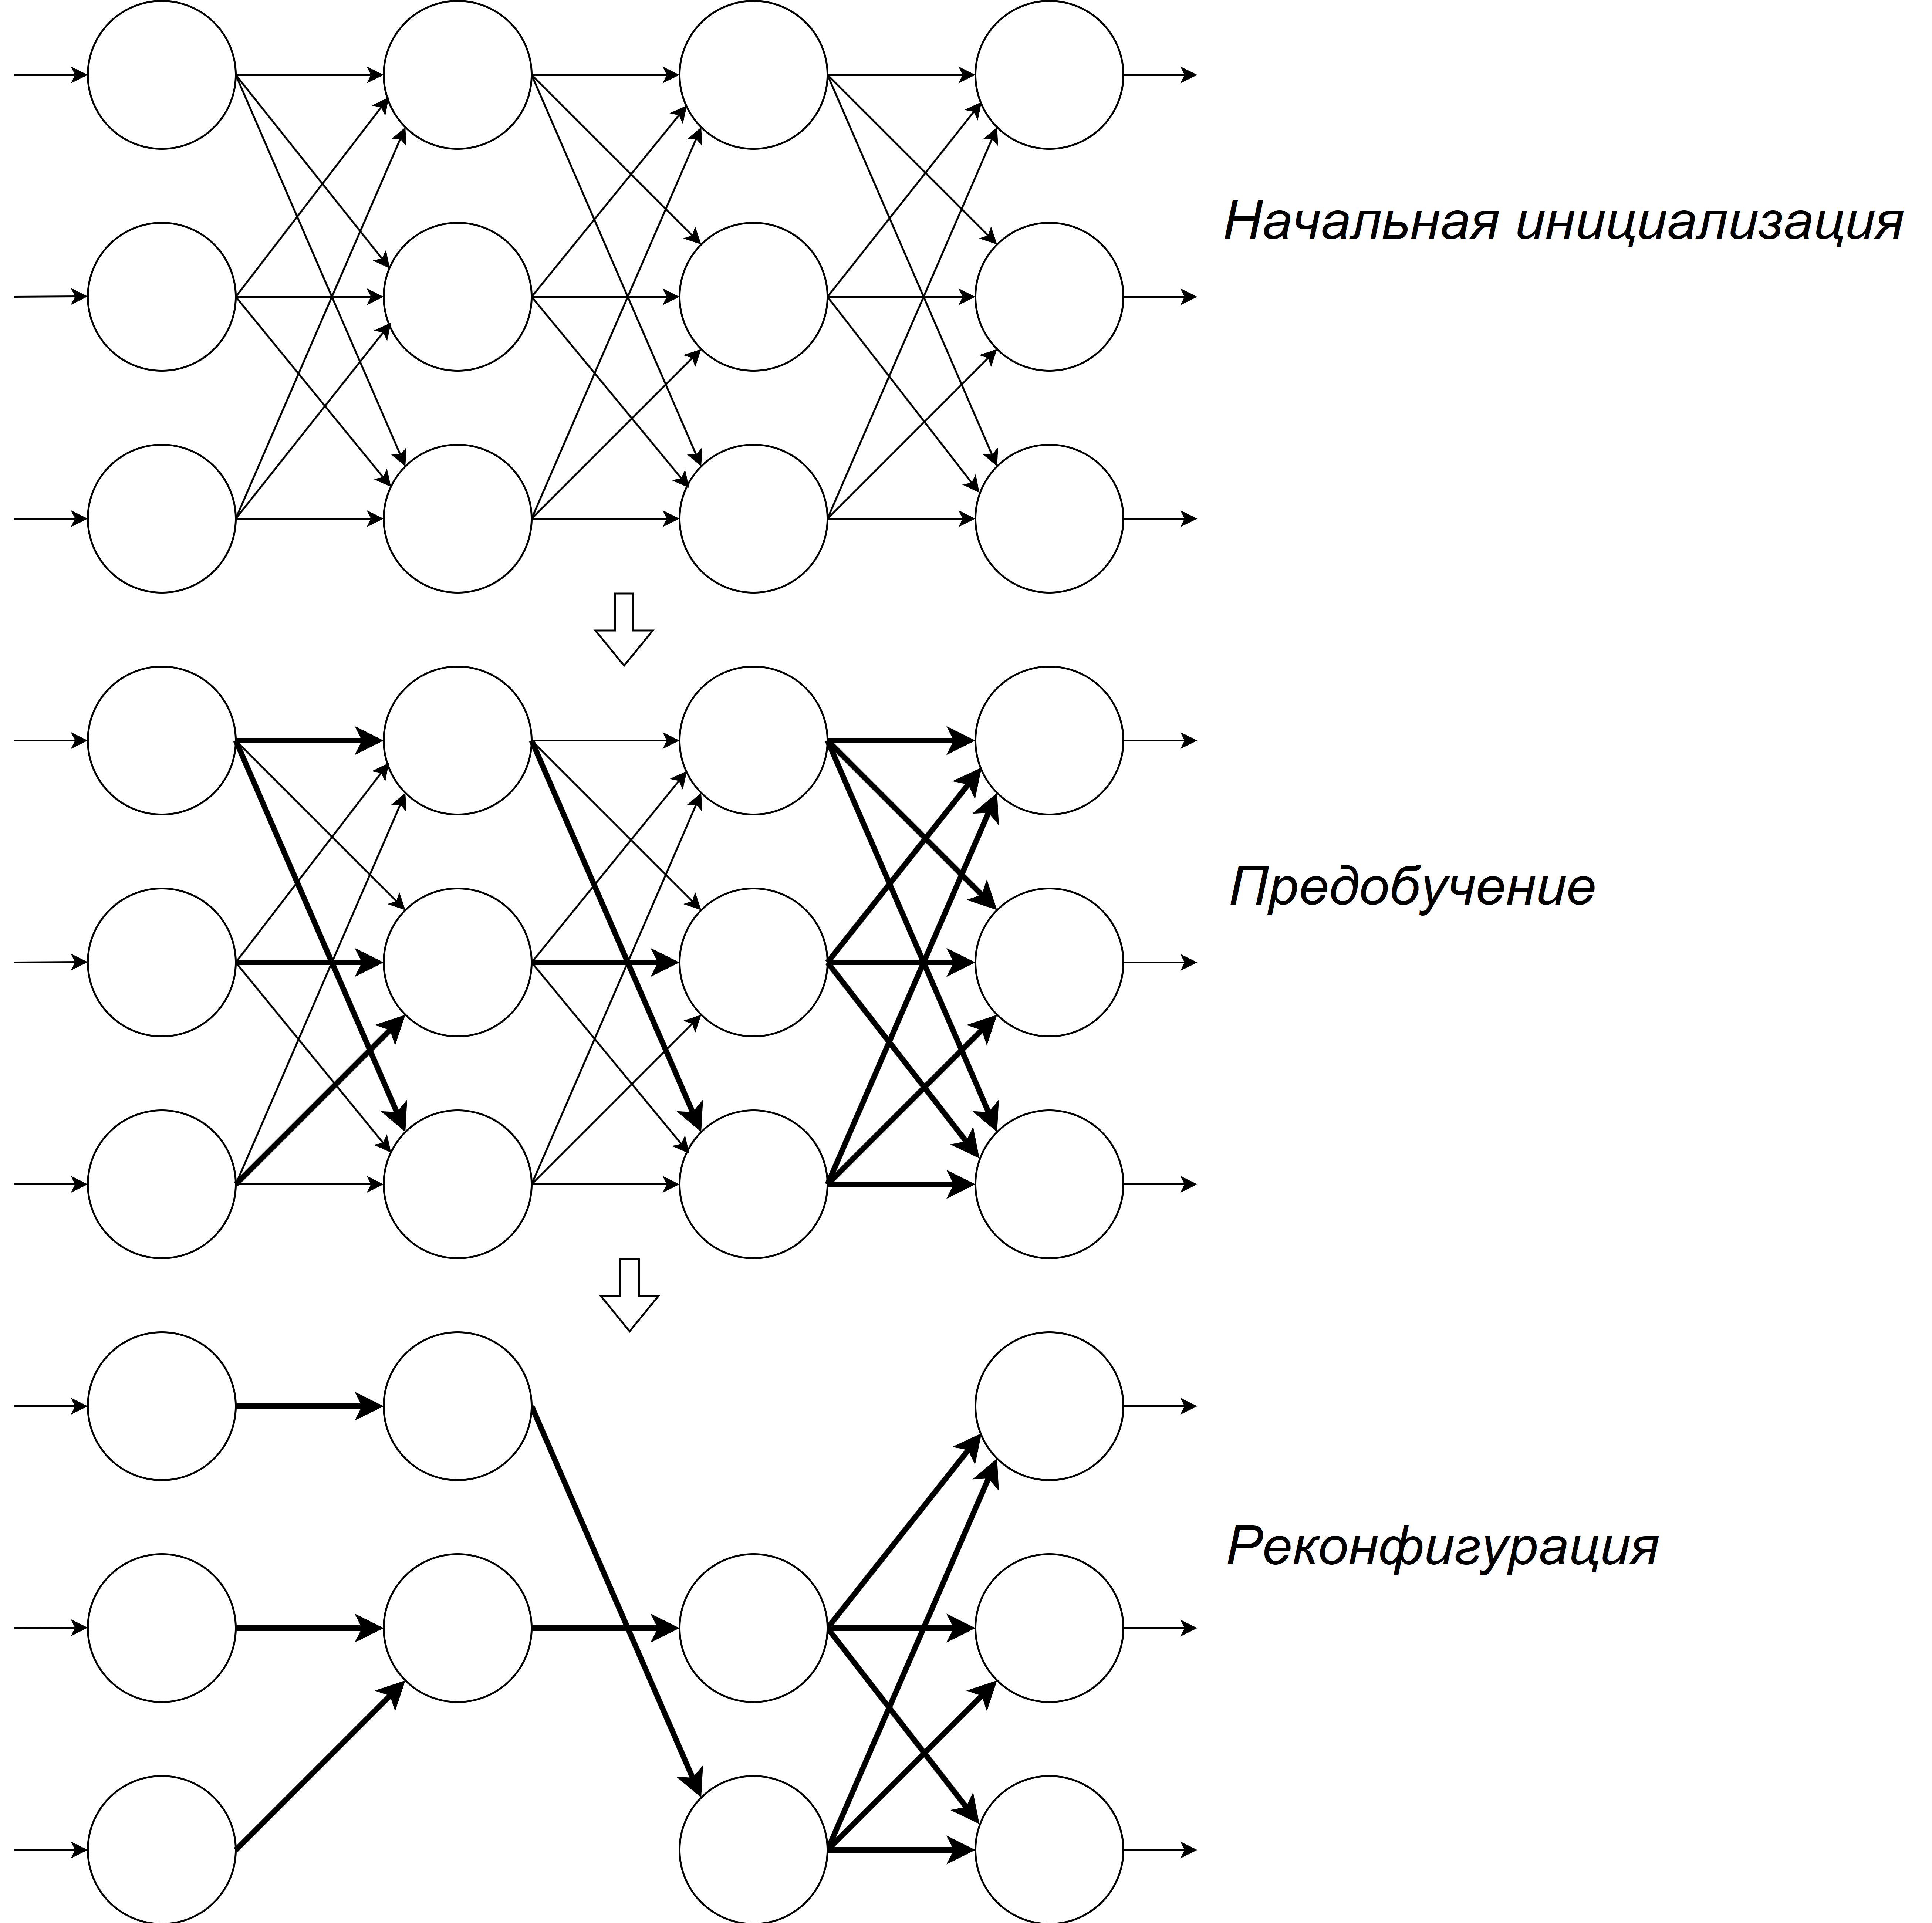
\includegraphics[width=0.7\textwidth]{man-source/images/ch2/pic2-3-1.png}
  \caption{Выполнение редуцирования весовых коэффициентов с архитектурной реконфигурацией НС}
  \label{fig:pic2_3}
\end{figure}

% Этап 3 метода редуцирования может быть представлен следующим алгоритмом:

% \begin{algo}[h]
% 	% \SetAlgoLined
	
% 	\KwIn{\textit{\textbf{x(0)}} -- вектор-образ из обучающей выборки,
% 		$\alpha$ - скорость обучения
% 	}
% 	\KwRes{матрица весовых коэффициентов \textit{\textbf{W}}, вектор порогов нейронов видимого слоя $\textit{\textbf{V}}$, вектор порогов нейронов скрытого слоя $\textit{\textbf{H}}$}
% 	\ForEach{нейрона скрытого слоя $j$}{
% 		Вычислить $P(y_{j}(0)=1|x_{i}(0))$ (для биномиальных нейронов sigmoid($\sum_{i}{w_{ij}x_{i}(0)}+H_j$))\;
% 		Генерировать $y_{j}(0) \in \{0, 1\}$ из $P(y_{j}(0)|x_i(0))$\;
% 	}
% 	\ForEach{нейрона видимого слоя $i$}
% 	{
% 		Вычислить $P(x_{i}(1)=1|y_j(0))$ (для биномиальных нейронов sigmoid($\sum_{j}{w_{ij}y_{j}(0)} + V_i$))\;
% 		Генерировать $x_{i}(1) \in \{0, 1\}$ из $P(x_{i}(1)|y_j(0))$\;
% 	}	
% 	\ForEach{скрытых нейронов $j$}
% 	{
% 		Вычислить $P(y_{j}(1)=1|x_i(1))$ (для биномиальных нейронов sigmoid($\sum_{i}{w_{ij}x_{i}(1)} + H_j$))\;
% 	}
% 	$\textit{\textbf{W}} \leftarrow \textit{\textbf{W}} + \alpha(\textbf{\textit{x(0)}}\textit{\textbf{y(0)}}^T - \textit{\textbf{x(1)}}P(\textit{\textbf{y(1)}}=1|\textit{\textbf{x(1)}})^T)$\;
% 	$\textit{\textbf{V}} \leftarrow \textit{\textbf{V}} + \alpha(\textit{\textbf{x(0)}} - \textit{\textbf{x(1)}})$\;
% 	$\textit{\textbf{H}} \leftarrow \textit{\textbf{H}} + \alpha(\textit{\textbf{y(0)}} - P(\textit{\textbf{y(1)}}=1|\textit{\textbf{x(1)}}))$\;
% %	\While{not at end of this document}{
% %		read current\;
% %		\eIf{understand}{
% %			go to next section\;
% %			current section becomes this one\;
% %		}{
% %		go back to the beginning of current section\;
% %	}
% %}
%     \caption{Процедура обучения RBM}
% 	\label{rbm_learning}
% \end{algo}

% \begin{figure}
% 	\begin{center}
% 		\includegraphics[width=120mm]{reducing_weights.png}
% 		\caption{Метод редуцирования весовых коэффициентов}				
% 		\label{reducing_weigths}
% 	\end{center}
% \end{figure}

% Согласно полученным экспериментальным данным, приведенным в главе \ref{chapt3}, выбор заданного порогового параметра на шаге 2 позволяет значительно упростить архитектуру нейронной сети, сократив количество параметров до 80\% относительно их исходного количества без существенных потерей в обобщающей способности нейронной сети. Данный метод наглядно демонстрирует высокую степень избыточности полносвязных архитектур, используемых для решения задач с небольшими обучающими выборками.

\section{Выводы}
\begin{easylistNum}
    & Предложен альтернативный подход к обучению ограниченной машины Больцмана, базирующийся на идее минимизации суммарной квадратичной ошибки восстановления образов на скрытом и видимом слоях. 
    & Доказана теорема об эквивалентности максимизации функции правдоподобия распределения входных данных \textit{P(x)} и минимизации суммарной квадратичной ошибки восстановления образов на скрытых и видимых слоях в одном и том же пространстве синаптических связей ограниченной машины Больцмана при использовании линейных нейронов.
    & Доказана теорема об эквивалентности максимизации функции правдоподобия распределения входных данных \textit{P(x)} минимизации кросс-энтропийной целевой функции $CE_s(k)$ в одном и том же пространстве синаптических весов ограниченной машины Больцмана (случаи CD-1 и CD-k).
    & Сформулирована обобщающая теорема об эквивалентности максимизации функции правдоподобия распределения входных данных P(x), минимизации кросс-энтропийной функции, минимизации суммарной квадратичной ошибки (специальный случай) в одном и том же пространстве синаптических весов ограниченной машины Больцмана.
    & Приведены правила обучения для различных случаев линейной и нелинейной машины Больцмана (RBM).
    % & Приведены правила обучения для нелинейной ограниченной машины Больцмана (случаи CD-1 и CD-k).
    % & Приведены правила группового обучения для линейной ограниченной машины Больцмана (случаи CD-1 и CD-k).
    % & Приведены правила группового обучения для нелинейной ограниченной машины Больцмана (случаи CD-1 и CD-k).
    & Приведены правила для обучения сверточных слоев ГНС с использованием модели CRBM.
    & Предложен метод редуцирования параметров глубокой полносвязной нейронной сети, основывающийся на использовании процедуры неконтролируемого предобучения слоев.
\end{easylistNum}
% \chapter{УНИФИЦИРОВАННЫЕ СЕМАНТИЧЕСКИЕ МОДЕЛИ ОБРАБОТКИ ЗНАНИЙ}

% %\addcontentsline{toc}{chapter}{\introname}	% Добавляем его в оглавление

% Общий принцип организации обработки информации, хранимой в семантической памяти ostis-системы, может быть иллюстрирован следующим образом (рисунок \ref{fig:pic_kpp}):
% \begin{figure}[H]
%   \centering
%   \includegraphics[width=\textwidth]{man-source/images/ch2/pic_kpp.jpg}
%   \caption{Организация обработки информации в ostis-системе}
%   \label{fig:pic_kpp}
% \end{figure}

% В соответствии с приведенной иллюстрацией объединенный решатель задач разделяется на платформенно зависимую часть (scp-интерпретатор) и платформенно независимую часть -- программу объединенного решателя. Программа решателя хранится в той же памяти, что и обрабатываемые знания, в той же памяти взаимодействуют и информационные процессы, выполняемые агентами решателя и направленные на решение каких либо задач. В рамках программы решателя выделяется модель операционной семантики языка SCP, т. е. модель scp-интерпретатора, которая реализуется в рамках платформы. В свою очередь, абстрактная sc-память реализуется в виде sc-хранилища. 

% Таким образом, в рамках данной главы основное внимание будет уделено:
% \begin{easylist}
% &	модели взаимодействия информационных процессов, выполняемых в семантической памяти, включающей классификацию таких процессов, механизмы регулирования их выполнения, средства решения различных конфликтов, в том числе связанных с параллельным выполнением таких процессов, средства спецификации состояния информационных процессов (выполняемый, отложенный, планирумеый и т. д.);
% &	агентно-ориентированной модели гибридного решателя задач, который является субъектом, выполняющим указанные информационные процессы и, соответственно, модель которого строится с учетом указанной модели взаимодействия информационных процессов.
% \end{easylist}

% Указанные модели тесно связаны между собой, в связи с чем задачи по их разработке разделяются на схожие подзадачи (рисунок~\ref{fig:pic2_1}).

% \begin{figure}[H]
%   \centering
%   \includegraphics[width=\textwidth]{man-source/images/ch2/pic2_1.pdf}
%   \caption{Структура главы 2}
%   \label{fig:pic2_1}
% \end{figure}

% В рамках технологии OSTIS основным средством спецификации предметных областей являются \textit{онтологии}. Представленная на рисунке \ref{fig:pic2_1} задачно-ориентированная спецификация определяет структуру данной главы диссертационного исследования, в рамках которой последовательно описываются:
% \begin{easylist}
% &	онтология действий и задач, уточняющая формальные средства спецификации преобразований, выполняемых различными субъектами в памяти компьютерной системы и за ее пределами;
% &	онтология действий в sc-памяти, уточняющая виды действий, выполняемых в такой памяти (информационных процессов);
% &	онтология sc-агентов, являющихся субъектами, выполняющими информационные процессы в sc-памяти;
% &	средства синхронизации выполнения параллельных информационных процессов в семантической памяти;
% &	онтология scp-программ, уточняющая понятие прогрраммы языка SCP, классификацию операторов языка SCP, средства их спецификации;
% &	агентно-ориентированная модель гибридного решателя задач, построенная на основе всех перечисленных онтологий;
% &	онтология интерпретатора scp-программ, который рассматривается как своего рода решатель задач частного вида и, соответственно, строится с использованием указанной выше модели. Данная онтология уточняет перечень агентов интерпретатора и их спецификацию.

% \end{easylist}

% Далее рассмотрим более подробно каждый из компонентов предложенной модели.
% \newpage
% \section[Формальная модель взаимодействия информационных процессов в семантической памяти]{Формальная модель взаимодействия информационных процессов\\ в семантической памяти}

% Формально модель взаимодействия информационных процессов в семантической памяти задается следующим образом:

% \begin{equation} 
% \label{<eq2_1>} 
% M_{IPM} = \{M_A, M_S, M_{SYNC}, M_{SCP}\},
% \end{equation} 

% \parindent=8mm
% \noindent \hangindent=22mm \hangafter=1
% где $M_A$ – модель деятельности, выполняемой различными субъектами (агентами) в памяти компьютерной системы и за ее пределами;

% \hangindent=22mm \hangafter=1
% $M_S$ – модель субъекта (агента), осуществляющего преобразования в семантической памяти компьютерной системы;

% \hangindent=30mm \hangafter=1
% $M_{SYNC}$ – модель синхронизации выполнения процессов в семантической памяти компьютерной системы;

% \hangindent=27mm \hangafter=1
% $M_{SCP}$ – модель базового языка программирования, ориентированного на обработку унифицированных семантических сетей, которая, в свою очередь, задается как

% \begin{equation} 
% \label{<eq2_2>} 
% M_{SCP} =\{M_P, M_I\},	
% \end{equation} 

% \noindent \hangindent=22mm \hangafter=1
% где $M_P$ – модель программы базового языка программирования;

% \hangindent=22mm \hangafter=1
% $M_I$ – модель интерпретатора программ базового языка программирования.

% \parindent=10mm

% Графическая иллюстрация модели взаимодействия процессов может быть приведена на рисунке \ref{fig:pic_proc_model}.

% \begin{figure}[H]
%   \centering
%   \includegraphics[width=0.7\textwidth]{man-source/images/ch2/pic_proc_model.pdf}
%   \caption{Модель взаимодействия процессов в семантической памяти}
%   \label{fig:pic_proc_model}
% \end{figure}

% Как видно из рисунка, в соответствии с изложенными ранее принципами агенты не обмениваются сообщениями напрямую, коммуникация между агентами осуществляется посредством спецификации выполняемых ими информационных процессов. В свою очередь, синхронизация выполнения параллельных информационных процессов осуществляется с использованием механизма блокировок элементов семантической памяти. Спецификация каждого информационного процесса фиксируется в семантической памяти. Каждый агент также имеет соответствующую спецификацию, которая является частью базы знаний системы и содержит сведения об условиях инициирования данного агента, возможных результатах его работы, ключевых элементах и т. д.

% Далее рассмотрим более подробно компоненты предложенной модели.

% \newpage
% \section{Формальные средства описания деятельности различных субъектов в семантической памяти} \label{section_actions}

% Модель деятельности, выполняемой различными субъектами (агентами) в памяти компьютерной системы и за ее пределами, задается следующим образом:

% \begin{equation} 
% \label{<eq2_3>} 
% M_A = \{A_C, A_{CM}, A_R, A_{CS}\},	
% \end{equation} 

% \parindent=8mm
% \noindent \hangindent=22mm \hangafter=1
% где $A_C$ – множество классов действий, выполняемых различными субъектами;

% \hangindent=25mm \hangafter=1
% $A_{CM}$ – множество классов действий, выполняемых агентами в семантической памяти, $A_{CM} \subset A_C$;

% \hangindent=22mm \hangafter=1
% $A_R$ – набор отношений, специфицирующих действия, принадлежащие классам из $A_C$;

% \hangindent=22mm \hangafter=1
% $A_{CS}$ – множество классов спецификаций действий, принадлежащих классам из $A_C$, таких как задача, протокол выполнения некоторого действия и т. д.;

% \parindent=10mm

% Более детально каждый компонент модели специфицируется в рамках \textit{предметной области действий и задач}. В рамках указанной предметной области исследуются такие общие понятия, как действие, субъект, объект действия, задача и ее решение и т. д. 

% Семантическая теория деятельности подробно рассматривается в работах В. В. Мартынова \cite{Martynov1974,Martynov1977,Martynov1984}, а также его учеников, в частности, в работе \cite{Boyko2016}. В указанных работах подробно рассматривается семантическая классификация действий, описываются подходы к формализации описания деятельности различного рода субъектов с использованием разработанного В. В. Мартыновым Универсального семантического кода (УСК). В этих работах детально рассматриваются такие понятия, как воздействие, субъект воздействия (агент), объект и другие, рассматриваемые также и в данной работе. 

% Кроме того, в работе \cite{Schenk1980} рассматриваются такие понятия, близкие рассматриваемым в данной работе, как воздействие, действие (акт), деятель (субъект) и другие.

% Задачей данной диссертационной работы, в отличие от указанных, является разработка средств описания деятельности различных субъектов в памяти компьютерной системы на основе SC-кода. Разработка таких средств позволит реализовать и интегрировать на их основе результаты, полученные в указанных работах, и использовать их в дальнейшем, в том числе при разработке различных решателей задач.

% \subsection{Общее понятие действия}

% В рамках предлагаемой модели описания деятельности понятие \textit{действие} является частным случаем понятия \textit{воздействие}, которое рассматривается в более общих предметных областях в рамках базы знаний IMS \cite{IMS2017}.
% В свою очередь, воздействие является частным случаем \textit{процесса}. Каждый \textit{процесс} определяется (задается) либо возникновением или исчезновением связей, связывающих заданную \textit{временную сущность} с другими сущностями, либо части указанной \textit{временной сущности} с другими сущностями. С точки зрения классификации фрагментов базы знаний \cite{Davydenko2016a} \textit{процесс} представляет собой ситуативную структуру, в каждый момент времени описывающую текущее состояние объектов, участвующих в данном процессе. \textit{Процесс}, описывающий изменения, происходящие исключительно в рамках sс-памяти, будем называть \textit{процессом в sc-памяти}.
% Каждому \textit{воздействию} может быть поставлена в соответствие 
% \begin{easylist}
% & некоторая \textit{воздействующая сущность* (субъект)}, т. е. сущность, осуществляющая воздействие (в частности, это может быть некоторое физическое поле);
% & некоторый \textit{объект воздействия*}, т. е. сущность, на которую воздействие направлено.
% \end{easylist}
% Если \textit{воздействие} связано с \textit{материальной сущностью}, то его объектом воздействия является либо сама эта \textit{материальная сущность}, либо некоторая ее пространственная часть.
% В свою очередь, каждое \textit{действие}, выполняемое тем или иным \textit{субъектом}, одновременно можно трактовать и как процесс решения некоторой задачи, т. е. как процесс достижения заданной цели в заданных условиях.
% Предполагается, что любое \textit{действие}, выполняемое каким-либо \textit{субъектом}, направлено на решение какой-либо задачи и выполняется \underline{целенаправленно}. При этом явное указание \textit{действия} и его связи с конкретной \textit{задачей} может не всегда присутствовать в памяти. Некоторые задачи могут решаться определенными агентами перманентно, например, оптимизация базы знаний, поиск некорректностей и т. д., и для подобных задач не всегда есть необходимость явно вводить \textit{структуру} \cite{Davydenko2016a}, являющуюся формулировкой \textit{задачи}.
% Каждое \textit{действие} обозначает некоторое преобразование, осуществляемое во внешней среде либо в памяти некоторой системы, однако в памяти явно вводятся только sc-элементы, обозначающие те \textit{действия}, для которых есть необходимость явно хранить их спецификацию в течение некоторого времени.
% При выполнении действия можно выделить следующие этапы:
% \begin{easylist}
% &	построение плана деятельности, декомпозиция исходного действия;
% &	выполнение построенного плана действий;
% \end{easylist}
% Формальная спецификация понятия действие в SCn-коде (в том числе – классификация действий с пояснениями) приведена в приложении \ref{AppendixActions}.

% В процессе описания в семантической памяти деятельности некоторого коллектива субъектов возникает необходимость выделять в рамках этой деятельности обособленные логически целостные фрагменты, которые могут выполняться отдельными субъектами независимо друг от друга.

% Спецификация понятия \textit{класса действий} в SCn-коде:

% \begin{flushleft}

% \noindent\setlength{\hangindent}{1em} 
% \hspace{-0.3em}\textbf{\itshape класс действий}\\
% $=${\itshape множество действий, однотипных в том или ином смысле}\\
% $<=$ {\itshape семейство подмножеств*}:\\
% \hspace{2em}{\itshape действие}\\
% $<=$ {\itshape разбиение*}:\\
% \hspace{2em}$\{$\\
% \hspace{3em}{$\bullet$ \itshape класс логически атомарных действий} \\
% \hspace{4em}$=${\itshape класс автономных действий}\\
% \hspace{3em}{$\bullet$ \itshape класс логически неатомарных действий} \\
% \hspace{4em}$=${\itshape класс неавтономных действий}\\
% \hspace{2em}$\}$
% \end{flushleft}

% Каждое \textit{действие}, принадлежащее некоторому конкретному \textit{классу логически атомарных действий}, обладает двумя необходимыми свойствами:
% \begin{easylist}
% & выполнение действия не зависит от того, является ли указанное действие частью декомпозиции более общего действия. При выполнении данного действия также не должен учитываться тот факт, что данное действие предшествует каким-либо другим действиям или следует за ними (что явно указывается при помощи отношения \textit{последовательность действий*});
% & указанное действие должно представлять собой логически целостный акт преобразования, например, в семантической памяти. Такое действие по сути является транзакцией, т. е. результатом такого преобразования становится новое состояние преобразуемой системы, а выполняемое действие должно быть либо выполнено полностью, либо не выполнено совсем, частичное выполнение не допускается. 
% \end{easylist}

% В то же время логическая атомарность не запрещает декомпозировать выполняемое действие на более частные, каждое из которых, в свою очередь, также будет являться логически атомарным. На рисунке \ref{fig:pic_laa} с использованием языка SCg показан пример декомпозиции более сложного логически атомарного действия на более простые.

% \begin{figure}[H]
%   \centering
%   \includegraphics[width=0.8\textwidth]{man-source/images/ch2/pic_laa.png}
%   \caption{Декомпозиция логически атомарного действия на поддействия}
%   \label{fig:pic_laa}
% \end{figure}

% На логически атомарные действия предлагается делить всю деятельность, направленную на решение каких-либо задач ostis-системой. Соответственно решатель предлагается делить на компоненты (агенты), соответствующие таким классам логически атомарных действий, что является основой для обеспечения его \textbf{модифицируемости}.

% В случае действий, выполняемых в семантической памяти, степень детализации каждого такого действия ограничивается синтаксическими особенностями используемого варианта представления знаний. В случае SC-кода можно выделить такие классы элементарных действий, как создание sc-элемента заданного типа, удаление sc-элемента, поиск sc-элементов, инцидентных указанному sc-элементу. На основе классификации таких элементарных преобразований в семантической памяти строится язык SCP, который описывается ниже в разделе~\ref{section_scp}.

% Предполагается, что каждое действие выполняется целенаправленно некоторым \textit{субъектом}. Формальная спецификация понятия \textit{субъект} в \mbox{SCn-коде} (в том числе – классификация субъектов):

% \begin{flushleft}

% \noindent\setlength{\hangindent}{1em} 
% \hspace{-0.3em}\textbf{\itshape субъект}\\
% $=${\itshape активная сущность}\\
% $=${\itshape сущность, способная самостоятельно выполнять некоторые виды действий}\\
% $=>$ {\itshape включение*}:\\
% \hspace{2em}{$\bullet$ \itshape собственное я ostis-системы} \\
% \hspace{2em}{$\bullet$ \itshape внутренний субъект ostis-системы} \\
% \setlength{\hangindent}{3em}
% \hspace{2em}{$\bullet$ \itshape внешний субъект ostis-системы, с которым осуществляется взаимодействие} \\
% \hspace{2em}{$\bullet$ \itshape внешний субъект ostis-системы, с которым взаимодействие не происходит} \\
% \end{flushleft}

% Под \textit{внутренним субъектом ostis-системы} понимается такой \textit{субъект}, который выполняет некоторые \textit{действия} в \underline{той же памяти}, в которой хранится его знак.

% К числу \textit{внутренних субъектов ostis-системы} относятся входящие в нее \textit{агенты}, отдельные решатели задач, целые интеллектуальные подсистемы.

% К числу \textit{внешних субъектов ostis-системы, с которыми осуществляется взаимодействие}, относятся конечные пользователи \textit{ostis-системы}, ее разработчики, а также другие компьютерные системы (причем, не только интеллектуальные).

% \subsection[Средства детализации процесса выполнения\\ действий]{Средства детализации процесса выполнения действий}

% Рассмотрим набор отношений, предназначенных для описания детализации процесса выполнения того или иного действия, т. е. выделения более простых частных действий.

% Связки отношения \textit{декомпозиция действия*} связывают \textit{действие} и множество частных \textit{действий}, на которые декомпозируется данное действие. При этом первым компонентом связки является знак указанного множества, вторым компонентом – знак более общего \textit{действия}.

% Таким образом, \textit{декомпозиция действия*} это \textit{квазибинарное отношение} \cite{IMS2017}, связывающее действие со множеством действий более низкого уровня, к выполнению которых сводится выполнение исходного декомпозируемого действия.

% Стоит отметить, что каждое \textit{действие} может иметь несколько вариантов декомпозиции в зависимости от конкретного набора элементарных действий, которые способна выполнять та или иная система \textit{субъектов}.

% Принцип, по которому осуществляется такая декомпозиция в различных подходах к решению задач, будем называть \underline{стратегией решения задач}.

% Кроме того, для детализации процесса выполнения действий используется отношение \textit{поддействие*}, связки которого связывают \textit{действие} и некоторое более простое частное \textit{действие}, выполнение которого необходимо для выполнения исходного более общего \textit{действия}.

% Для описания порядка выполнения действий используется отношение \textit{последовательность действий*}, частными видами которого являются отношения \textit{последовательность действий при положительном результате*} и \textit{последовательность действий при отрицательном результате*}.

% Связки отношения \textit{последовательность действий*} связывают знаки \textit{действий}, выполняющихся в какой-либо последовательности в процессе решения какой-либо задачи. При этом считается, что если два \textit{действия} связаны данным отношением, то \textit{действие}, стоящее в данной связке на втором месте, может быть выполнено только после выполнения действия, стоящего в данной связке на первом месте. Таким образом, каждое действие может быть инициировано после завершения выполнения любого из предшествующих действий.

% Переход по связкам отношения \textit{последовательность действий при положительном результате*} от предшествующего действия проверки условия к последующему действию происходит при условии, если указанная проверка даст положительный результат, т. е. предшествующее действие станет \textit{успешно выполненным действием}.

% Переход по связкам отношения \textit{последовательность действий при отрицательном результате*} от предшествующего действия проверки условия к последующему действию происходит при условии, если указанная проверка даст отрицательный результат, т. е. предшествующее действие станет \textit{безуспешно выполненным действием}.

% Для обеспечения возможности синхронизации выполнения действий используется класс действий \textit{конъюнкция предшествующих действий}. Действия указанного класса используются в тех случаях, когда выполнение некоторого действия должно начаться только после того, как будут выполнены все предшествующие действия, а не только одно из них. После того как все предшествующие действия выполнены, инициируются действия, следующие за \textit{конъюнкцией предшествующих действий}.

% В некоторых случаях бывает необходимо управлять процессом выполнения какой-либо последовательности действий в зависимости от выполнения дополнительных условий. Для осуществления таких проверок вводится класс действий \textit{проверки условия}. Действия класса \textit{проверка условия} предполагают проверку истинности или ложности некоторого высказывания (условия), и после выполнения в зависимости от результата данной проверки становятся \textit{успешно выполненными действиями} или \textit{безуспешно выполненными действиями}.

% Следует отметить, что предлагаемый подход к описанию переходов между действиями очень близок к решениям, описанным в уже упоминавшейся статье \cite{Kotov1966}. Действительно, каждое действие независимо от его сложности можно считать аналогом процессорного элемента, рассмотренного в указанной статье, а условием инициирования какого-либо действия (спусковой функцией) является факт завершенности хотя бы одного из предыдущих действий (т. е. связанных с текущим действием связкой отношения \textit{последовательность действий*} или более частных отношений). Таким образом, использование предлагаемого языка описания деятельности различных субъектов на различных уровнях позволит не только говорить об универсальности и «понятности» такого описания за счет использования самых базовых понятий, но и о возможности реализации различных моделей \underline{параллелизма на любом уровне}, начиная от параллельного выполнения операторов в рамках одной программы, заканчивая взаимодействием целых коллективов агентов в общей семантической памяти. Возможность реализации той или иной модели параллелизма в таком случае определяется исключительно особенностями решаемой задачи.


% \subsection{Спецификация действий}
% Важнейшим с точки зрения функционирования системы понятием является понятие задачи. Под \textit{задачей} понимается формальная спецификация некоторого действия (условие), достаточная для выполнения данного действия каким-либо \textit{субъектом}. В зависимости от конкретного класса задач описываться может как внутреннее состояние самой интеллектуальной системы, так и требуемое состояние внешней среды. \textit{sc-элемент}, обозначающий \textit{действие}, входит в \textit{задачу} под атрибутом \textit{ключевой sc-элемент'}.

% Классификация задач может осуществляться по дидактическому признаку в рамках каждой предметной области, например, задачи на треугольники, задачи на системы уравнений и т. п.

% Каждая \textit{задача} может включать:
% \begin{easylist}
% &	факт принадлежности \textit{действия} какому-либо частному классу \textit{действий} (например, \textit{действие. сформировать полную семантическую окрестность указываемой сущности}), в том числе состояние \textit{действия} с точки зрения жизненного цикла (инициированное, выполняемое и т. д.);
% &	описание \textit{цели* (результата*) действия}, если она точно известна;
% &	указание \textit{заказчика* действия};
% &	указание \textit{исполнителя* действия} (в том числе коллективного);
% &	указание \textit{аргумента(ов) действия’};
% &	указание инструмента или посредника \textit{действия};
% &	описание \textit{декомпозиции действия*};
% &	указание \textit{последовательности действий*} в рамках \textit{декомпозиции действия*}, т.е построение плана решения задачи. Другими словами, построение плана решения представляет собой декомпозицию соответствующего \textit{действия} на систему взаимосвязанных между собой поддействий;
% &	указание области \textit{действия};
% &	указание условия инициирования действия;
% &	момент начала и завершения \textit{действия}, в том числе планируемый и фактический, предполагаемая и/или фактическая длительность выполнения.

% \end{easylist}

% Некоторые задачи могут быть дополнительно уточнены контекстом – дополнительной информацией о сущностях, рассматриваемых в формулировке \textit{задачи}, т. е. описанием того, что дано, что известно об указанных сущностях.

% Кроме этого, \textit{задача} может включать любую дополнительную информацию о действии, например:
% \begin{easylist}
% &	перечень ресурсов и средств, которые предполагается использовать при решении задачи, например, список доступных исполнителей, временные сроки, объем имеющихся финансов и т. д.;
% &	ограничение области, в которой выполняется действие, например, необходимо заменить одну sc-конструкцию на другую по некоторому правилу, но только в пределах некоторого раздела базы знаний;
% &	ограничение знаний, которые можно использовать для решения той или иной задачи, например, необходимо решить задачу по алгебре, используя только те утверждения, которые входят в курс школьной программы до седьмого класса включительно, и не используя утверждения, изучаемые в старших классах;
% &	и прочее.
% \end{easylist}
% С одной стороны, решаемые системой задачи можно классифицировать на \textit{информационные задачи} и \textit{поведенческие задачи}. 

% С точки зрения формулировки поставленной задачи можно выделить \textit{декларативные формулировки задачи} и \textit{процедурные формулировки задачи}. Следует отметить, что данные классы задач не противопоставляются, и могут существовать формулировки задач, использующие оба подхода.

% В случае \textit{процедурной формулировки задачи} в формулировке задачи явно указываются аргументы соответствующего задаче \textit{действия} и, в частности, вводится семантическая классификация \textit{действий}. При этом явно не уточняется, что должно быть результатом выполнения данного действия. Заметим, что при необходимости \textit{процедурная формулировка задачи} может быть сведена к \textit{декларативной формулировке задачи} путем трансляции на основе некоторого правила, например, определения класса действия через более общий класс.

% В случае \textit{декларативной формулировки задачи} при описании условия задачи специфицируется цель \textit{действия}, т. е. результат, который должен быть получен при успешном выполнении \textit{действия}.

% В свою очередь, под \textit{вопросом} понимается задача, направленная на удовлетворение информационной потребности некоторого субъекта-заказчика.

% Под \textit{командой} (в том числе – \textit{интерфейсной командой}) понимается спецификация инициированного действия (инициированная задача).

% Рассмотрим набор отношений, используемых для формальной спецификации действий в рамках \textit{задачи}.

% Связки отношения \textit{результат*} связывают \textit{sc-элемент}, обозначающий \textit{действие}, и \textit{sc-конструкцию}, описывающую результат выполнения рассматриваемого действия, другими словами, цель, которая должна быть достигнута при выполнении \textit{действия}.

% Результат может специфицироваться как атомарным высказыванием, так и неатомарным, т. е. конъюнктивным, дизъюнктивным, строго дизъюнктивным и т. д.
% В случае, когда успешное выполнение \textit{действия} приводит к изменению какой-либо конструкции в \textit{sc-памяти}, которое необходимо занести в историю изменений базы знаний или использовать для демонстрации протокола решения задачи, генерируется соответствующая связка отношения \textit{результат*}, связывающая \textit{задачу} и \textit{sc-конструкцию}, описывающую данное изменение. Конкретный вид указанной \textit{sc-конструкции} зависит от типа действия.

% Связки отношения \textit{исполнитель*} связывают \textit{sc-элементы}, обозначающие \textit{действие} и \textit{sc-элементы}, обозначающие \textit{субъекта}, который предположительно будет осуществлять, осуществляет или осуществлял выполнение указанного \textit{действия}. Данное отношение может быть использовано при назначении конкретного исполнителя для проектной задачи по развитию баз знаний.

% В случае, когда заранее неизвестно, какой именно \textit{субъект*} будет исполнителем данного \textit{действия}, связка отношения \textit{исполнитель*} может отсутствовать в первоначальной формулировке \textit{задачи} и добавляться позже, уже непосредственно при исполнении.

% Когда действие выполняется (является \textit{настоящей сущностью}) или уже выполнено (является \textit{прошлой сущностью}), то исполнитель этого действия в каждый момент времени уже определен.

% Связки отношения \textit{заказчик*} связывают \textit{sc-элементы}, обозначающие \textit{действие}, и \textit{sc-элементы}, обозначающие \textit{субъекта}, который <<заинтересован>> в выполнении данного действия и, как правило, инициирует его выполнение. Данное отношение может быть использовано при указании того, кто поставил проектную задачу по развитию базы знаний.

% Связки отношения \textit{объект*} связывают \textit{sc-элемент}, обозначающий \textit{действие}, и знак той сущности, над которой (по отношению к которой) осуществляется данное \textit{действие}, например, знак \textit{структуры}, подлежащий верификации.

% Связки отношения \textit{контекст действия*} связывают \textit{sc-элементы}, обозначающие \textit{действие} и \textit{структуры}, обозначающие контекст выполнения данного \textit{действия}, т. е. некоторую дополнительную информации о тех сущностях, которые входят в описание \textit{цели*}. Как правило, контекст используется для указания собственно условия некоторой задачи, того, что дано, т. е. тех знаний, которые можно использовать для вывода новых знаний при решении задачи. Таким образом, контекст непосредственно влияет на то, как будет решаться та или иная задача, при этом даже задачи, соответствующие одному классу действий, могут решаться по-разному.

% Контекст может быть представлен не только в виде атомарного фактографического высказывания, но и в виде высказывания более сложного вида. Это может быть, например:
% \begin{easylist}
% &	определение множества, используемого в описании \textit{цели*};
% &	утверждение, учет которого может быть полезен в решении задач.
% \end{easylist}
% В случае процедурной формулировки задачи для указания в рамках конкретного действия тех sc-элементов, над которыми непосредственно выполняется данное действие, используется ролевое отношение \textit{аргумент действия'}.

% Для уточнения класса сущностей, которые могут быть аргументами действий, соответствующих некоторому \textit{классу команд}, используется отношение \textit{класс аргументов*}. В случае, когда \textit{команды} данного класса имеют один аргумент, используется собственно отношение \textit{класс аргументов*}, в случае, когда больше команды данного класса имеют более одного аргумента, то используются подмножества данного отношения, такие, как \textit{класс первых аргументов*}, \textit{класс вторых аргументов*} и т. д.

% На рисунке \ref{fig:pic_probl_ex} с использованием языка SCg показан пример представления задачи в sc-памяти, связанной с установлением истинности высказывания о конгруэнтности двух треугольников.

% \begin{figure}[H]
%   \centering
%   \includegraphics[width=0.85\textwidth]{man-source/images/ch2/pic_probl_ex.png}
%   \caption{Пример представления задачи}
%   \label{fig:pic_probl_ex}
% \end{figure}

% Если для некоторого \textit{класса команд} не указан тип какого-либо из аргументов, то предполагается, что в качестве данного аргумента может выступать любой \textit{sc-элемент}.

% Кроме задачи как спецификации действия в целом необходимо выделить еще ряд \textit{семантических окрестностей} \cite{Davydenko2016a}, специфицирующих конкретное действие с той или иной стороны.

% \begin{easylist}
% &	План выполнения действия

% Каждый \textit{план} представляет собой \textit{семантическую окрестность}, ключевым \textit{sc-элементом'} является \textit{действие}, для которого дополнительно детализируется предполагаемый процесс его выполнения. Основная задача такой детализации – локализация области базы знаний, в которой предполагается работать, а также набора агентов, необходимого для выполнения описываемого действия. При этом детализация необязательно должна быть доведена до уровня элементарных действий, цель составления плана – уточнение подхода к решению той или иной задачи, не всегда предполагающее составления подробного пошагового решения.

% При описании \textit{плана} может быть использован как процедурный, так и декларативный подход. В случае процедурного подхода для соответствующего \textit{действия} указывается его декомпозиция на более частные поддействия, а также необходимая спецификация этих поддействий. В случае декларативного подхода указывается набор подцелей (например, при помощи логических утверждений), достижение которых необходимо для выполнения рассматриваемого \textit{действия}. На практике оба рассмотренных подхода можно комбинировать.

% В общем случае \textit{план} может содержать и переменные, например, в случае, когда часть плана задается в виде цикла (многократного повторения некоторого набора действий). Также план может содержать константы, значение которых в настоящий момент не установлено и станет известно, например, только после выполнения предшествующих ему \textit{действий}.

% Каждый \textit{план} может быть задан заранее как часть спецификации \textit{действия}, т. е. задачи, а может формироваться \textit{субъектом} уже собственно в процессе выполнения \textit{действия}, например, в случае использования стратегии разбиения задачи на подзадачи. В первом случае \textit{план включается*} в \textit{задачу}, соответствующую тому же действию.

% &	Программа выполнения класса действий

% Каждая \textit{программа} представляет собой обобщенный \textit{план} выполнения \textit{действий}, принадлежащих некоторому классу, т. е. \textit{семантическую окрестность}, \textit{ключевым sc-элементом'} является \textit{класс действий}, для элементов которого дополнительно детализируется процесс их выполнения.

% В остальном описание программы аналогично описанию \textit{плана} выполнения конкретного \textit{действия} из рассматриваемого \textit{класса действий}.

% Одному \textit{классу действий} может соответствовать несколько \textit{программ}.

% Входным параметрам \textit{программы} в традиционном понимании соответствуют аргументы, соответствующие каждому \textit{действию} из \textit{класса действий}, описываемого \textit{программой}. При генерации на основе \textit{программы плана} выполнения конкретного \textit{действия} из данного класса эти аргументы принимают конкретные значения.

% Каждая \textit{программа} представляет собой систему описанных действий с дополнительным указанием для действия:

% &	либо \textit{последовательности выполнения действий*} (передачи инициирования), когда условием выполнения (инициирования) действий является завершение выполнения одного из указанных или всех указанных действий;
% &	либо события в базе знаний или внешней среде, являющегося условием его инициирования;
% &	либо ситуации в базе знаний или внешней среде, являющейся условием его инициирования.
% \end{easylist}

% Видно, что предложенная трактовка понятия программы как обобщенного плана выполнения некоторого класса действий никак не ограничивает область его применения, в частности, как программа в таком смысле может трактоваться рецепт приготовления какого-либо блюда, обобщенное описание какого-либо технологического процесса, инструкция по использованию какого-либо устройства и т. д.

% Пример программы \textit{языка SCP} (scp-программы) представлен в приложении \ref{AppendixSCP} (рисунок \ref{img:examplescp1}). Более подробно сам \textit{язык SCP} будет рассмотрен ниже.

% Данный пример представляет собой \textit{scp-программу}, имеющую два аргумента (множество и элемент, который надо добавить во множество). В соответствии с алгоритмом программы осуществляется проверка того, имеется ли указанный элемент в указанном множестве, и если нет, то элемент добавляется во множество. В рамках данной программы исходный scp-процесс декомпозируется на три более простых подпроцесса (\textit{поддействия*}), связанных соответствующими подклассами отношения \textit{последовательность выполнения действий*}. Таким образом, программа состоит из трех элементарных действий (\textit{scp-операторов}) – поиск элемента во множестве, добавление элемента во множество и завершение выполнения, между которыми указаны два условных перехода и один безусловный. Часть используемых в данном примере понятий идентифицирована при помощи \textit{системных идентификаторов*} \cite{IMS2017}, например, \textit{nrel\_then, nrel\_else} и т. д.

% Кроме того, выделяются такие классы \textit{семантических окрестностей} действий, как \textit{протокол} выполнения действия, содержащий декомпозицию рассматриваемого \textit{действия} на поддействия с указанием порядка их выполнения, а также необходимой спецификацией каждого такого поддействия, и решение, в рамках которого указываются только те поддействия, без которых решение поставленной задачи было бы невозможным, т. е. из \textit{протокола} исключаются ложные или избыточные шаги, проделанные в процессе поиска пути решения задачи, которые, в свою очередь, могут присутствовать при описании непосредственно текущего хода решения задачи.

% \subsection{Классификация действий в семантической памяти} \label{section_actions_in_sc_memory}
% Отдельное внимание следует уделить действиям, выполняемым в семантической памяти компьютерной системы (sc-памяти).

% Описанные в данном подразделе понятия исследуются в рамках \textit{предметной области действий, выполняемых в абстрактной унифицированной семантической памяти} и представлены в соответствующем разделе базы знаний метасистемы IMS \cite{IMS2017}.

% Каждое \textit{действие в sc-памяти} обозначает некоторое преобразование, выполняемое некоторым \textit{субъектом} (или коллективом \textit{субъектов}) в рамках \mbox{\textit{sc-памяти}}. Спецификация действия после его выполнения может быть включена в протокол решения некоторой задачи. 

% Семантика каждого \textit{действия в sc-памяти} зависит от конкретного контекста, т. е. ориентации действия на какие-либо конкретные объекты и принадлежности действия какому-либо конкретному классу действий.

% Следует четко отличать:
% \begin{easylist}
% &	каждое конкретное \textit{действие в sc-памяти}, представляющее собой некоторый переходный процесс, переводящий sc-память из одного состояния в другое;
% &	каждый тип \textit{действий в sc-памяти}, представляющий собой некоторый класс однотипных (в том или ином смысле) действий;
% &	sc-узел, обозначающий некоторое конкретное \textit{действие в sc-памяти};
% &	sc-узел, обозначающий структуру, которая является описанием, спецификацией, заданием, постановкой соответствующего действия.

% \end{easylist}

% Формальная спецификация понятия действие в sc-памяти на языке SCn:

% \begin{flushleft}

% \noindent\setlength{\hangindent}{1em} 
% \hspace{-0.3em}\textbf{\itshape действие в sc-памяти}\\
% $=${\itshape внутреннее действие ostis-системы}\\
% $=${\itshape действие, выполняемое в sc-памяти}\\
% $=${\itshape действие, выполняемое решателем задач ostis-системы}\\
% $<=$ {\itshape включение*}:\\
% \hspace{2em}{\itshape процесс в sc-памяти} \\
% $=>$ {\itshape включение*}:\\
% \hspace{2em}{$\bullet$ \itshape действие в sc-памяти, инициируемое вопросом} \\
% \hspace{2em}{$\bullet$ \itshape действие редактирования базы знаний ostis-системы} \\
% \hspace{2em}{$\bullet$ \itshape действие установки режима ostis-системы} \\
% \hspace{2em}{$\bullet$ \itshape действие редактирования файла, хранимого в sc-памяти} \\
% \hspace{2em}{$\bullet$ \itshape действие интерпретации программы, хранимой в sc-памяти} \\
% \end{flushleft}

% Формальная спецификация понятия \textit{действие в sc-памяти, инициируемое вопросом}, представлена в приложении \ref{AppendixActionsByQuest} на языке SCn. Формальная спецификация понятия \textit{действие редактирования базы знаний} на языке SCn представлена в приложении \ref{AppendixActionsEditing}.

% \newpage
% \section{Модель субъекта, осуществляющего преобразования в рамках общей семантической памяти} \label{section_agents}

% \subsection{Понятие абстрактного sc-агента и их семантическая классификация}

% Единственным видом \textit{субъектов}, выполняющих преобразования в \mbox{\textit{sc-памяти}}, будем считать \textit{sc-агенты}. Для формального определения понятия \textit{sc-агента} воспользуемся введенным ранее понятием \textit{класса логически атомарных действий}. Будем называть \textit{sc-агентом} некоторый \textit{субъект}, способный выполнять \textit{действия в sc-памяти}, принадлежащие некоторому определенному \textit{классу логически атомарных действий}.

% Формально модель субъекта (агента), осуществляющего преобразования в семантической памяти компьютерной системы задается следующим образом:

% \begin{equation} 
% \label{<eq2_4>} 
% M_S = \{S_C, S_R\},	
% \end{equation} 
% где $S_C$ – множество классов (видов) sc-агентов;

% \parindent=8mm
% $S_R$ – набор отношений, заданных на множестве sc-агентов.
% \parindent=10mm

% Логическая атомарность выполняемых sc-агентом действий предполагает, что каждый sc-агент реагирует на соответствующий ему класс ситуаций \mbox{и/или} событий, происходящих в sc-памяти, и осуществляет определенное преобразование sc-текста (текста SC-кода), находящегося в семантической окрестности обрабатываемой ситуации и/или события. При этом каждый sc-агент в общем случае не имеет информацию о том, какие еще sc-агенты в данный момент присутствуют в системе и осуществляет взаимодействие в другими \mbox{sc-агентами} исключительно посредством формирования некоторых конструкций (как правило – спецификаций действий) в общей sc-памяти. Таким сообщением может быть, например, вопрос, адресованный другим sc-агентам в системе (заранее не известно, каким конкретно), или ответ на поставленный другими sc-агентами вопрос (опять же, не известно, каким конкретно). Таким образом, каждый sc-агент в каждый момент времени контролирует только фрагмент базы знаний в контексте решаемой данным агентом задачи, состояние всей остальной базы знаний в общем случае непредсказуемо для sc-агента. 

% Важно отметить, что конечный пользователь ostis-системы с логической точки зрения также выступает в процессе обработки знаний как sc-агент, формирующий в sc-памяти сообщения путем выполнения элементарных действий, предусмотренных пользовательским интерфейсом. Аналогичным образом осуществляется взаимодействие ostis-системы с другими системами и окружающей средой вообще. Вся информация поступает в ostis-систему и из ostis-системы исключительно посредством соответствующих sc-агентов интерфейса.

% Описанные в данном разделе понятия исследуются в рамках \textit{предметной области абстрактных агентов, работающих над унифицированной семантической памятью}, и представлены в соответствующем разделе базы знаний метасистемы IMS \cite{IMS2017}.

% Перечислим некоторые достоинства предлагаемого подхода к организации обработки знаний в sc-памяти:
% \begin{easylist}
% &	поскольку обработка осуществляется агентами, которые обмениваются сообщениями \underline{только} через общую память, добавление нового агента или исключение (деактивация) одного или нескольких существующих агентов, как правило, не приводит к изменениям в других агентах, поскольку агенты не обмениваются сообщениями напрямую;
% &	инициирование агентов осуществляется децентрализованно и чаще всего независимо друг от друга, таким образом, даже существенное расширение числа агентов в рамках одной системы не приводит к ухудшению ее производительности;
% &	спецификации агентов и, как будет показано ниже, их программы могут быть записаны на том же языке, что и обрабатываемые знания, что существенно сокращает перечень специализированных средств, предназначенных для проектирования таких агентов и их коллективов, а также их анализа, верификации и оптимизации, и упрощает разработку системы за счет использования более универсальных компонентов.

% \end{easylist}

% %\textcolor{red}{РОЛИК ПРО ВЗАИМОДЕЙСТВИЕ АГЕНТОВ}

% Поскольку предполагается, что копии одного и того же \textit{sc-агента} или функционально эквивалентные \textit{sc-агенты} могут работать в разных ostis-системах, будучи при этом физически разными sc-агентами, то целесообразно рассматривать свойства и классификацию не sc-агентов, а классов функционально эквивалентных sc-агентов, которые будем называть \textit{абстрактными sc-агентами}.

% Таким образом, под \textit{абстрактным sc-агентом} понимается некоторый класс функционально эквивалентных \textit{sc-агентов}, разные экземпляры (т. е. представители) которого могут быть реализованы по-разному.

% Каждый \textit{абстрактный sc-агент} имеет соответствующую ему спецификацию. В спецификацию каждого \textit{абстрактного sc-агента} входит:
% \begin{easylist}
% &	указание ключевых \textit{sc-элементов} \textit{sc-агента}, т. е. тех \textit{\mbox{sc-элементов}}, хранимых в \textit{sc-памяти}, которые для него являются <<точками опоры>>;
% &	формальное описание условий инициирования \textit{sc-агента}, т. е. тех \textit{ситуаций} в \textit{sc-памяти}, которые инициируют деятельность данного \mbox{\textit{sc-агента}};
% &	формальное описание первичного условия инициирования \textit{sc-агента}, \mbox{т. е.} такой ситуации в \textit{sc-памяти}, которая побуждает \textit{sc-агента} перейти в активное состояние и начать проверку наличия своего полного условия инициирования;
% &	строгое, полное, однозначно понимаемое описание деятельности данного \textit{sc-агента}, оформленное при помощи каких-либо понятных, общепринятых средств, не требующих специального изучения, например на естественном языке;
% &	описание результатов выполнения работы соответствующих \mbox{\textit{sc-агентов}}.

% \end{easylist}

% Первичным условием инициирования некоторого sc-агента может быть некоторое элементарное изменение (событие) в семантической памяти, число которых ограничено. Рассмотрим классификацию таких элементарных событий в SCn-коде:
% \begin{flushleft}

% \noindent\setlength{\hangindent}{1em} 
% \hspace{-0.3em}\textbf{\itshape элементарное событие в sc-памяти*}\\

% $<=$ {\itshape разбиение*}:\\
% \hspace{2em}{$\{$\itshape } \\

% \hspace{2em}{$\bullet$ \itshape событие добавления sc-дуги, выходящей из заданного sc-элемента*} \\
% \hspace{2em}{$\bullet$ \itshape событие добавления sc-дуги, входящей в заданный sc-элемент*} \\
% \hspace{2em}{$\bullet$ \itshape событие добавления sc-ребра, инцидентного заданному sc-элементу*} \\
% \hspace{2em}{$\bullet$ \itshape событие удаления sc-дуги, выходящей из заданного sc-элемента*} \\
% \hspace{2em}{$\bullet$ \itshape событие удаления sc-дуги, входящей в заданный sc-элемент*} \\
% \hspace{2em}{$\bullet$ \itshape событие удаления sc-ребра, инцидентного заданному sc-элементу*} \\
% \hspace{2em}{$\bullet$ \itshape событие удаления sc-элемента*} \\
% \hspace{2em}{$\bullet$ \itshape событие изменения содержимого файла*} \\
% \hspace{2em}{$\}$\itshape } \\
% \end{flushleft}

% Для того чтобы иметь возможность рассмотреть полную классификацию \textit{абстрактных sc-агентов}, выделяемую в настоящее время, следует уделить внимание языку программирования SCP, который используется в качестве базового языка для описания программ обработки текстов \textit{SC-кода}, в том числе -- программ, реализующих алгоритмы работы \textit{sc-агентов}.

% \textit{Язык SCP} – это графовый язык процедурного программирования, предназначенный для эффективной обработки однородных семантических сетей с теоретико-множественной интерпретацией, закодированных с помощью \textit{\mbox{SC-кода}}. \textit{Язык SCP} является языком параллельного асинхронного программирования.

% Языком представления данных для текстов \textit{языка SCP (scp-программ)} является \textit{SC-код}. Данный факт позволяет обеспечить независимость программ, реализованных на \textit{языке SCP}, от платформы интерпретации sc-моделей, в связи с чем программы большинства sc-агентов предполагается реализовывать именно на указанном языке. Однако очевидно, что в таком случае в системе должны также существовать реализованные на платформенно-зависимом уровне \textit{sc-агенты}, осуществляющие интерпретацию scp-программ. Данное ограничение учитывается в представленной ниже классификации \textit{абстрактных sc-агентов}.

% Классификация \textit{абстрактных sc-агентов}, записанная в SCn-коде, представлена в приложении \ref{AppendixAgents}.

% С точки зрения реализации можно выделить два класса \textit{абстрактных \mbox{sc-агентов}}:
% \begin{easylist}
% &	под \textit{неатомарным абстрактным sc-агентом} понимается \textit{абстрактный sc-агент}, который декомпозируется на коллектив более простых \textit{абстрактных sc-агентов}, каждый из которых в свою очередь может быть как \textit{атомарным абстрактным \mbox{sc-агентом}}, так и \textit{неатомарным абстрактным \mbox{sc-агентом}}. При этом в каком-либо варианте \textit{декомпозиции абстрактного sc-агента*} дочерний \textit{неатомарный абстрактный \mbox{sc-агент}} может стать \textit{атомарным абстрактным \mbox{sc-агентом}} и реализовываться соответствующим образом;
% &	под \textit{атомарным абстрактным sc-агентом} понимается абстрактный sc-агент, для которого уточняется платформа его реализации, т. е. существует соответствующая связка отношения \textit{программа sc-агента*}.
% \end{easylist}

% В свою очередь, \textit{атомарные абстрактные sc-агенты} подразделяются на \textit{платформенно-независимые абстрактные sc-агенты} и \textit{платформенно-зависимые абстрактные sc-агенты}.

% К \textit{платформенно-независимым абстрактным sc-агентам} относят \textit{атомарные абстрактные sc-агенты}, реализованные на \textit{языке SCP}.

% При описании \textit{платформенно-независимых абстрактных sc-агентов} под платформенной независимостью понимается платформенная независимость с точки зрения технологии OSTIS, т.е реализация на языке SCP, поскольку \textit{атомарные sc-агенты}, реализованные на указанном языке, могут свободно переноситься с одной платформы интерпретации sc-моделей на другую.

% К \textit{платформенно-зависимым абстрактным sc-агентам} относят \textit{атомарные абстрактные sc-агенты}, реализованные ниже уровня sc-моделей, т. е. не на \textit{языке SCP}, а на каком-либо другом языке описания программ.

% Существуют \textit{sc-агенты}, которые принципиально должны быть реализованы на платформенно-зависимом уровне, например, собственно \textit{sc-агенты} интерпретатора \textit{языка SCP} или рецепторные и эффекторные \textit{sc-агенты}, обеспечивающие взаимодействие с внешней средой.

% По отношению к внешней среде \textit{абстрактные sc-агенты} могут быть \textit{внутренними абстрактными sc-агентами, эффекторными абстрактными \mbox{sc-агентами}, рецепторными абстрактными \mbox{sc-агентами}}.

% Каждый \textit{внутренний абстрактный sc-агент} обозначает класс \textit{sc-агентов}, которые реагируют на события в \textit{sc-памяти} и осуществляют преобразования исключительно в рамках этой же \textit{sc-памяти}.

% Каждый \textit{эффекторный абстрактный sc-агент} обозначает класс \textit{\mbox{sc-агентов}}, которые реагируют на события в \textit{sc-памяти} и осуществляют преобразования во внешней относительно данной \textit{ostis-системы} среде.

% Каждый \textit{рецепторный абстрактный sc-агент} обозначает класс \textit{\mbox{sc-агентов}}, которые реагируют на события во внешней относительно данной \textit{ostis-системы} среде и осуществляют преобразования в памяти данной системы.

% Как было сказано выше, существуют \textit{абстрактные sc-агенты}, которые принципиально не могут быть реализованы на языке SCP. С данной точки зрения можно выделить два соответствующих класса \textit{абстрактных sc-агентов}:
% \begin{easylist}
% &	каждый \textit{абстрактный sc-агент, не реализуемый на языке SCP}, должен быть реализован на уровне платформы интерпретации sc-моделей, в том числе, аппаратной. К таким \textit{абстрактным sc-агентам} относятся абстрактные \mbox{sc-агенты} интерпретации scp-программ, а также эффекторные и рецепторные абстрактные sc-агенты;
% &	каждый \textit{абстрактный sc-агент, реализуемый на языке SCP}, может быть реализован на \textit{языке SCP}, т. е. платформенно-независимом уровне, но при необходимости может реализовываться и на уровне платформы, например, с целью повышения производительности.
% \end{easylist}

% Отдельное внимание следует уделить классификации абстрактных \mbox{sc-агентов} с точки зрения используемых средств синхронизации деятельности sc-агентов того или иного класса. По данному критерию выделяются три класса абстрактных sc-агентов:
% \begin{easylist}
% &	к \textit{абстрактным sc-агентам интерпретации scp-программ} относятся не реализуемые на платформенно-независимом уровне \textit{абстрактные sc-агенты}, обеспечивающие интерпретацию \textit{scp-программ} и \textit{scp-метапрограмм}, в том числе создание \textit{scp-процессов}, собственно интерпретацию \textit{scp-операторов}, а также другие вспомогательные действия. По сути, агенты данного класса обеспечивают работу sc-агентов более высоких уровней (программных \mbox{sc-агентов} и sc-метаагентов), реализованных на языке SCP, в частности, обеспечивают соблюдение указанными агентами общих принципов синхронизации, которые будут изложены ниже;
% &	к \textit{абстрактным программным sc-агентам} относятся все \textit{абстрактные sc-агенты}, обеспечивающие основную функциональность системы, т. е. ее возможность решать те или иные задачи. Агенты данного класса должны работать в соответствии с общими принципами синхронизации деятельности субъектов в sc-памяти;
% &	задачей \textit{абстрактных sc-метаагентов} является координация деятельности \textit{абстрактных программных sc-агентов} (точнее, их элементов, т. е. конкретных \textit{программных sc-агентов}), в частности, решение проблемы взаимоблокировок (подробно механизмы синхронизации выполнения параллельных процессов в sc-памяти рассмотрены ниже в соответствующем разделе.). Агенты данного класса могут быть реализованы на \textit{языке SCP}, однако для синхронизации их деятельности используются другие принципы, соответственно, для реализации таких агентов требуется \textit{язык SCP} другого уровня, классификация операторов которого полностью аналогична классификации \textit{\mbox{scp-операторов}}, однако эти операторы имеют другую операционную семантику, учитывающую отличия в принципах синхронизации (работы с \textit{блокировками*}). Программы такого языка будем называть \textit{scp-метапрограммами}, соответствующие им \textit{процессы в sc-памяти} – \textit{scp-метапроцессами}, операторы – \textit{scp-метаоператорами}.
% \end{easylist}

% Классификация \textit{sc-агентов} по отношению к платформе интерпретации \mbox{sc-моделей}, внешней среде ostis-системы и средствам синхронизации их деятельности полностью аналогична соответствующей классификации \textit{абстрактных sc-агентов}, в связи с чем не будем отдельно рассматривать такую классификацию.

% Дополнительно вводится класс \textit{активных sc-агентов}. Под \textit{активным \mbox{sc-агентом}} понимается \textit{sc-агент} ostis-системы, который реагирует на события, соответствующие его условию инициирования, и, как следствие, его \textit{первичному условию инициирования*}. Не входящие во множество \textit{активных \mbox{sc-агентов} \mbox{sc-агенты}} не реагируют ни на какие события в \textit{sc-памяти}.

% Для описания деятельности sc-агентов в sc-памяти вводится понятие процесса и процесса в sc-памяти, которые будут рассмотрены ниже.

% Классификация sc-агентов по семантике выполняемых ими преобразований в sc-памяти будет представлена ниже в разделе, посвященном классификации решателей задач.

% \subsection{Формальные средства спецификации абстрактных \mbox{sc-агентов}}

% Как было сказано выше, каждый абстрактный sc-агент должен быть специфицирован соответствующим образом, в противном случае функционирование соответствующих sc-агентов станет невозможным. Рассмотрим ряд отношений, используемых для спецификации абстрактных sc-агентов.

% Связки отношения \textit{ключевые sc-элементы sc-агента*} связывают между собой \textit{sc-узел}, обозначающий \textit{абстрактный sc-агент}, и \textit{sc-узел}, обозначающий множество \textit{sc-элементов}, которые являются ключевыми для данного \textit{абстрактного sc-агента}, т. е. данные \textit{sc-элементы} являются элементами программ, реализующих данный \textit{абстрактный sc-агент}.

% Связки отношения \textit{программа sc-агента*} связывают между собой \textit{\mbox{sc-узел}}, обозначающий \textit{атомарный абстрактный sc-агент}, и \textit{sc-узел}, обозначающий множество программ, реализующих указанный \textit{атомарный абстрактный \mbox{sc-агент}}.

% В случае \textit{платформенно-независимого абстрактного sc-агента} каждая связка отношения \textit{программа sc-агента*} связывает \textit{sc-узел}, обозначающий указанный \textit{абстрактный sc-агент}, с множеством \textit{scp-программ}, описывающих деятельность данного \textit{абстрактного sc-агента}. Данное множество содержит одну \textit{агентную scp-программу} и произвольное количество (может быть, и ни одной) \textit{scp-программ}, которые необходимы для выполнения указанной \textit{агентной scp-программы}. Понятие \textit{агентной scp-программы} будет подробнее рассмотрено ниже.

% В случае \textit{платформенно-зависимого абстрактного sc-агента} каждая связка отношения \textit{программа sc-агента*} связывает \textit{sc-узел}, обозначающий указанный \textit{абстрактный sc-агент} с множеством файлов, содержащих исходные тексты программы на некотором внешнем языке программирования, реализующей деятельность данного \textit{абстрактного sc-агента}.

% Связки отношения \textit{первичное условие инициирования*} связывают между собой \textit{sc-узел}, обозначающий \textit{абстрактный sc-агент}, и бинарную ориентированную пару, описывающую первичное условие инициирования данного \textit{абстрактного sc-агента}, т. е. такую спецификацию \textit{ситуации} в \textit{sc-памяти}, возникновение которой побуждает \textit{sc-агента} перейти в активное состояние и начать проверку наличия своего полного условия инициирования.

% После того как в \textit{sc-памяти} происходит некоторое событие, активизируются все \textit{активные sc-агенты, первичное условие инициирования*} которых соответствует произошедшему событию.

% Связки отношения \textit{условие инициирования и результат*} связывают между собой \textit{sc-узел}, обозначающий \textit{абстрактный sc-агент}, и бинарную ориентированную пару, связывающую условие инициирования данного \textit{абстрактного sc-агента} и результаты выполнения экземпляров данного sc-агента в какой-либо конкретной системе.

% Указанную ориентированную пару можно рассматривать как логическую связку импликации, при этом на \textit{sc-переменные}, присутствующие в обеих частях связки, неявно накладывается квантор всеобщности, на \textit{sc-переменные}, присутствующие либо только в посылке, либо только в заключении, неявно накладывается квантор существования.

% Кроме описанных отношений спецификация \textit{абстрактного sc-агента} также включает \textit{описание поведения sc-агента}, которое представляет собой \textit{семантическую окрестность} \cite{Davydenko2016a}, описывающую деятельность sc-агента до какой-либо степени детализации, однако такое описание должно быть строгим, полным и однозначно понимаемым. Как любая другая \textit{семантическая окрестность, описание поведения sc-агента} может быть протранслировано на какие-либо понятные, общепринятые средства, не требующие специального изучения, например, на естественный язык.

% Описываемый \textit{абстрактный sc-агент} входит в соответствующее \textit{описание поведения sc-агента} под атрибутом \textit{ключевой sc-элемент'}.

% Строго говоря, для того чтобы элементы некоторого \textit{абстрактного \mbox{sc-агента}} (конкретные \textit{sc-агенты}) могли работать (реагировать на соответствующие события в sc-памяти и выполнять соответствующую программу), достаточно описать \textit{первичное условие инициирования*} и \textit{программу \mbox{sc-агента}*} для данного абстрактного sc-агента. Остальные фрагменты спецификации могут быть использованы для дополнительного анализа соответствующего агента другими агентами, для дидактических целей и т. д.

% Пример формальной спецификации \textit{абстрактного sc-агента} на примере \textit{абстрактного sc-агента поиска структуры, изоморфной заданному образцу}, приведен в приложении \ref{AppendixAgentSpec}.

% \newpage
% \section[Формальные средства спецификации действий базовой машины обработки унифицированных семантических\\ сетей]{Формальные средства спецификации действий базовой машины обработки унифицированных семантических сетей} \label{section_scp}

% В качестве базового языка для описания программ, реализующих деятельность sc-агентов в рамках \textit{sc-памяти} предлагается \textit{язык SCP}, разрабатываемый в рамках технологии OSTIS. \textit{Язык SCP} ориентирован на обработку унифицированных семантических сетей, представленных в \textit{SC-коде}.

% Базовая модель обработки текстов \textit{SC-кода} включает в себя:
% \begin{easylist}
% &	модель предметной области \textit{scp-программ}, в которую включаются все тексты \textit{scp-программ}, в которой исследуется классификация операторов этих программ и средства их спецификации;
% &	модель предметной области агентов интерпретатора \textit{scp-программ (Абстрактной scp-машины)}, который является частью платформы интерпретации sc-моделей. Термин \textit{абстрактная} в данном случае, как и в случае с \textit{абстрактным sc-агентом}, показывает, что разрабатывается семантическая модель scp-интерпретатора, включающая спецификацию каждого из агентов в его составе, которая может в дальнейшем быть реализована в рамках какой-либо платформы интерпретации sc-моделей, в том числе, аппаратной.
% \end{easylist}

% Собственно разработка \textit{языка SCP} не являлась задачей данной диссертационной работы, поскольку данный язык был разработан ранее и подробно описан, например, в работах \cite{Golenkov1996,Golenkov1995a,Golenkov1995b,Golenkov1994e,Golenkov1994b,Golenkov1994c,Golenkov1994a,Golenkov1994d}.

% Одной из задач данной диссертационной работы является построение указанных выше моделей предметных областей и соответствующих им онтологий, а также включение разработанных моделей в базу знаний метасистемы IMS. 

% Актуальность данной задачи обсусловлена следующими факторами:
% \begin{easylist}
% &	формализация и представление в базе знаний указанных моделей обеспечит возможность легко модифицировать указанные модели при необходимости, в том числе:
% &&	автоматизировать процесс изменения и верификации самих моделей;
% &&	упростить процесс приведения существующих компонентов к новым версиям языка SCP за счет локализации изменений и автоматизации указанного процесса;
% &	включение указанных моделей в базу знаний IMS позволит обеспечить информационную поддержку разработчиков и снизить предъявляемые к ним требования, за счет:
% &&	автоматизации поиска нужной справочной информации, упрощение навигации по справочным материалам, возможность локализации необходимой в текущий момент информации;
% &&	возможности снабжения разработанных моделей различного рода обучающей информацией, примерами, пояснениями, упражнениями и т. д., другими словами -- возможность построения развитых средств обучения языку SCP;
% &	результат построения указанных моделей, т. е. полное формальное описания денотационной и операционной семантики языка SCP представляет собой, по сути, строгое техническое задание на разработку \textit{платформ интерпретации sc-моделей} как в программном варианте, так и в \underline{аппаратном}. 

% \end{easylist}

% Построение указанных онтологий потребовало уточнения некоторых понятий языка SCP, а также принципов интерпретации scp-программ, в частности, потребовалось решить некоторые дополнительные задачи, представленные ниже:

% \textbf{Привести онтологию языка SCP в соответствие с общей онтологией описания деятельности различных субъектов}, представленной в соответствующем разделе данной диссертационной работы. В частности, \mbox{scp-программа} должна трактоваться как частный случай программы, \mbox{scp-оператор} -- как частный случай действия в sc-памяти, scp-процесс -- как частный случай процесса в sc-памяти. Решение данной задачи, во-первых, позволит сократить количество ключевых sc-элементов, уникальных для онтологии языка SCP, и, соответственно, упростить его изучение, во-вторых, обеспечит возможность построения на базе языка SCP языков, операторы которых описывают более сложные преобразования в sc-памяти, при этом общие принципы интерпретации останутся неизменными. Кроме того, при таком подходе при каждой новой попытке интерпретации scp-программы будет создаваться отдельный независимый scp-процесс, являющийся, по сути, копией scp-программы с учетом известных входных данных. Такой подход к интерпретации имеет ряд достоинств, о которых будет сказано ниже.

% Операторы языка SCP (\textit{scp-операторы}) трактуются как знаки элементарных действий в sc-памяти, которые должны интерпретироваться интерпретатором scp-программ, который является частью \textit{платформы интерпретации sc-моделей}.
% В свою очередь, \textit{scp-процесс} трактуется как некоторое \textit{действие в sc-памяти}, в декомпозиции которого могут присутствовать только знаки \mbox{scp-операторов}. Данный факт гарантирует, что каждый \textit{scp-процесс} может быть интерпретирован интерпретатором \textit{scp-программ}.

% \textbf{Выделить два уровня языка SCP}, первый из которых обеспечит возможность реализации программных sc-агентов (т. е. уровень, использующий предлагаемый ниже механизм блокировок), второй – sc-метаагентов (т. е. уровень, не использующий механизм блокировок). Операторы языка второго уровня во многом аналогичны операторам языка первого уровня, однако они имеют другую операционную семантику, которая не учитывает блокировки и в рамках которой они рассматриваются как обычные конструкции SC-кода. Данный факт позволяет сделать следующие выводы: 
% \begin{easylist}
% &	поскольку блокировки в данном случае будут обрабатываться так же, как любые другие конструкции в sc-памяти, то такой язык позволит реализовывать программы sc-метаагентов, в задачи которых входит и анализ блокировок;
% &	операционная семантика языка SCP первого уровня, т. е. собственно языка реализации программных sc-агентов, учитывающая блокировки, может быть описана с использованием языка SCP второго уровня. В связи с этим упомянутый язык второго уровня будем считать языком микропрограмм языка SCP. Наличие языка микропрограмм, операционная семантика которого проще, чем у собственно языка SCP, позволит упростить и аппаратную реализацию языка SCP как ассемблера для упомянутого выше ассоциативного графодинамического компьютера.

% \end{easylist}

% \textbf{Построить модель интерпретатора языка SCP}, которая бы обладала следующими основными особенностями:

% \begin{easylist}
% &	интерпретатор языка SCP представляет собой, по сути, решатель частного частного вида и должен быть построен на базе общей модели гибридного решателя задач, которая будет уточнена ниже. При этом принципы взаимодействия агентов интерпретации sсp-программ упрощаются за счет создания независимого scp-процесса для каждого акта выполнения scp-программы, а также за счет ограниченности набора таких агентов, алгоритм работы каждого из которых известен;
% &	новая версия интерпретатора языка SCP должна обеспечивать интерпретацию обоих рассмотренных выше уровней языка SCP. Интерпретация языка SCP первого уровня подразумевает обеспечение на уровне интерпретатора соблюдения всех принципов синхронизации деятельности sc-агентов, описанных в соответствующем разделе.
% \end{easylist}

% В ряде диссертационных работ по смежной тематике, представленных ранее, также рассматривались понятия scp-процесса, принципы интерпретации scp-программ, механизмы синхронизации выполнения scp-процессов, в частности, в работах \cite{Gaponov2000,Ivashenko1999}.

% Можно указать следующие основные отличия описываемой диссертационной работы от указанных:

% \begin{easylist}
% &	по сравнению с работой \cite{Gaponov2000} минимизировано число блокировок, алгоритмы работы с ними детализированы до уровня элементарных преобразований в sc-памяти, классификация блокировок основана на общей классификации структур в sc-памяти, описанной в работе \cite{Davydenko2016a};
% &	введены отношения \textit{планируемая блокировка*}, \textit{приоритет блокировки*} и \textit{удаляемые sc-элементы*}, таким образом, явно показано, как в рамках механизма синхронизации обрабатываются ситуации, когда какой-либо информационный процесс в sc-памяти пытается получить доступ к \mbox{sc-элементам}, заблокированным другим процессом;
% &	описаны причины возникновения взаимоблокировок, разработаны механизмы борьбы с ними, в частности, введено понятие sc-метаагента;
% &	выделен минимально необходимый набор транзакций, которые должны быть реализованы на уровне платформы интерпретации sc-моделей для того, чтобы полностью обеспечить описанные механизмы работы с блокировками;
% &	разработан новый механизм интерпретации scp-программ, предполагающий создание независимого scp-процесса для каждого акта выполнения \mbox{scp-программы}. Преимущества данного механизма рассмотрены ниже;
% &	предлагаемые решения ориентированы на работу в общей единой семантической памяти, выделение каких-либо частей в которой осуществляется исключительно средствами SC-кода, а не на уровне технической реализации платформы интерпретации sc-моделей;
% &	изменена семантическая трактовка понятия scp-процесса, \mbox{scp-программы}, процесса в sc-памяти. Таким образом, понятие scp-процесса интегрируется в общую онтологию деятельности, что позволяет минимизировать число специализированных средств, необходимых для спецификации scp-процессов и синхронизации их выполнения.

% \end{easylist}

% В рамках базовой модели обработки текстов \textit{SC-кода} выделяются дополнительные классы \textit{структур} (sc-конструкций) \cite{Davydenko2016a}, на работу с которыми ориентированы те или другие классы \textit{scp-операторов}. Классификация и примеры таких структур приведены в 
% приложении \ref{AppendixStructures}.

% \subsection{Понятие scp-программы и scp-процесса}

% Каждая \textit{scp-программа} представляет собой \textit{обобщенную структуру}, описывающую один из вариантов декомпозиции действий некоторого класса, выполняемых в sc-памяти. Знак \textit{sc-переменной}, соответствующей конкретному декомпозируемому действию, является в рамках \textit{scp-программы ключевым \mbox{sc-элементом'}}. Также явно указывается принадлежность данного знака множеству \textit{scp-процессов}.

% Таким образом, каждая \textit{scp-программа} описывает в обобщенном виде декомпозицию некоторого \textit{scp-процесса} на взаимосвязанные \textit{scp-операторы} с указанием аргументов для данного \textit{scp-процесса} при их наличии.

% По сути каждая \textit{scp-программа} представляет собой описание последовательности элементарных операций, которые необходимо выполнить над семантической сетью, чтобы выполнить более сложное действие некоторого класса.

% Частным случаем \textit{scp-программ} являются \textit{агентные scp-программы. \mbox{Scp-программы}} данного класса представляют собой реализации программ агентов обработки знаний и имеют жестко фиксированный набор параметров. Каждая такая программа имеет ровно два \textit{in-параметра’} (данное понятие описано ниже). Значение первого параметра является знаком бинарной ориентированной пары, являющееся вторым компонентом связки отношения \textit{первичное условие инициирования*} для абстрактного \textit{sc-агента}, в множество \textit{программ sc-агента*} которого входит рассматриваемая \textit{агентная scp-программа}.

% Значением второго параметра является \textit{sc-элемент}, с которым непосредственно связано событие, в результате возникновения которого был инициирован соответствующий \textit{sc-агент}, т. е., например, сгенерированная либо удаляемая \textit{sc-дуга} или \textit{sc-ребро}.

% В свою очередь, под \textit{scp-процессом} понимается некоторое \textit{действие в sc-памяти}, однозначно описывающее конкретный акт выполнения некоторой \textit{scp-программы} для заданных исходных данных. Если \textit{scp-программа} описывает алгоритм решения какой-либо задачи в общем виде, то \textit{scp-процесс} обозначает конкретное действие, реализующее данный алгоритм для заданных входных параметров. 

% По сути \textit{scp-процесс} представляет собой копию, созданную на основе \textit{scp-программы}, в которой каждой \textit{sc-переменной}, за исключением \textit{\mbox{scp-переменных'}}, соответствует сгенерированная \textit{sc-константа}.

% Принадлежность некоторого действия множеству \textit{scp-процессов} по определению гарантирует тот факт, что в декомпозиции данного действия будут присутствовать только знаки элементарных действий (\textit{scp-операторов}), которые может интерпретировать scp-интерпретатор.

% Пример выполнения scp-процесса, соответствующего scp-программе добавления элемента в канторовское множество, представлен в \mbox{приложении \ref{AppendixSCP}}. На рисунках \ref{img:examplescp2}--\ref{img:examplescp5} последовательно показаны состояния процесса в \mbox{sc-памяти}, соответствующие разным этапам его выполнения. В рассмотренном примере считается, что заданный элемент ранее не содержался в заданном множестве и будет добавлен в него после выполнения scp-процесса.

% \subsection[Спецификация действий базовой машины\\ обработки]{Спецификация действий базовой машины обработки}

% Каждый \textit{scp-оператор} представляет собой некоторое элементарное \textit{действие в sc-памяти}. Аргументы \textit{scp-оператора} будем называть операндами. Порядок операндов указывается при помощи соответствующих ролевых отношений (\textit{1’, 2’, 3’} и т. д.). Операнд, помеченный ролевым отношением \textit{1’}, будем называть первым операндом и т. д., помеченный ролевым отношением \textit{2’} -- вторым операндом и т. д. Тип и смысл каждого операнда также уточняется при помощи различных подклассов отношения \textit{scp-операнд'}. В общем случае операндом может быть любой \textit{sc-элемент}, в том числе знак какой-либо \textit{scp-программы}, в том числе самой программы, содержащей данный оператор. Полная классификация scp-операндов в SCn-коде с пояснениями приведена в приложении \ref{AppendixSCPOperands}.

% Каждый \textit{scp-оператор} должен иметь один и более операнд. Кроме того, при помощи соответствующих отношений (\textit{последовательность действий*} и более частных) должен быть указан тот \textit{scp-оператор} (или несколько scp-операторов), который должен быть выполнен следующим. Исключение из данного правила составляет \textit{scp-оператор завершения выполнения программы}, который не содержит ни одного операнда и после выполнения которого никакие \textit{scp-операторы} в рамках данной программы выполняться не могут.

% Выделяется также множество \textit{атомарный тип scp-оператора}, каждый элемент которого представляет собой класс \textit{scp-операторов}, который не разбивается на более частные, и, соответственно, напрямую интерпретируется реализацией \textit{Абстрактной scp-машины}.

% В приложении \ref{AppendixSCPOperators} приведена полная классификация \textit{scp-операторов}, представленная в SCn-коде (нижние уровни в каждом из классов являются \textit{атомарными типами scp-операторов}).

% Введение класса \textit{scp-оператор обработки содержимых файлов} необходимо для обеспечения возможности реализации на языке SCP рецепторных и эффекторных \textit{sc-агентов}.

% Ролевое отношение \textit{начальный оператор'} указывает в рамках декомпозиции соответствующего \textit{scp-программе} действия те поддействия, которые должны быть выполнены в первую очередь, т. е. те, с которых собственно начинается выполнение \textit{scp-процесса}.

% Как было сказано выше, соответствующий \textit{scp-программе scp-процесс} может иметь один и более параметров, каждый из которых имеет свой номер (\textit{1’, 2’} и т. д.). В настоящее время выделены два класса параметров (в SCn-коде):

% \begin{flushleft}

% \noindent\setlength{\hangindent}{1em} 
% \hspace{-0.3em}\textbf{\itshape параметр scp-программы'}\\
% $<=$ {\itshape  включение*}:\\
% \hspace{2em}{\itshape аргумент действия'}:\\
% $<=$ {\itshape разбиение*}:\\
% \hspace{2em}{$\{$\itshape } \\


% \hspace{2em}{$\bullet$ \itshape in-параметр’} \\
% \hspace{2em}{$\bullet$ \itshape out-параметр’} \\
% \hspace{2em}{$\}$\itshape } \\
% \end{flushleft}

% Параметры типа \textit{in-параметр'} хоть и соответствуют \textit{переменным \mbox{scp-программы’}}, не могут менять значение в процессе ее интерпретации. Фиксированное значение переменной устанавливается при создании уникальной копии \textit{scp-программы (scp-процесса)} для ее интерпретации, и, таким образом, соответствующая scp-переменная' на момент начала ее интерпретации становится \textit{scp-константой'} в рамках каждого \textit{scp-оператора}, в котором встречалась данная \textit{scp-переменная'}. Использование \textit{in-параметров} можно рассматривать по аналогии с использованием варианта механизма передачи по значению в традиционных языках программирования, с тем условием что значение локальной переменной в рамках дочерней программы не может быть изменено.

% Параметры типа \textit{out-параметр'} соответствуют \textit{переменным \mbox{scp-программы'}} и обладают всеми теми же соответствующими свойствами. Чаще всего предполагается, что значение данного параметра необходимо родительской \textit{scp-программе}, содержащей оператор вызова текущей \textit{\mbox{scp-программы}}. При этом на момент начала интерпретации в качестве параметра дочернему процессу передается непосредственно узел, обозначающий переменную (а точнее, ее уникальную копию в рамках процесса) родительского процесса. Указанная переменная может при необходимости иметь значение либо не иметь. После завершения и во время интерпретации дочернего процесса родительский процесс по-прежнему может работать с переменной, переданной в качестве \textit{out-параметра'}, при необходимости просматривая или изменяя ее значение. Использование out-параметра можно рассматривать по аналогии с использованием механизма передачи по ссылке в традиционных языках программирования.

% \subsection{Достоинства базовой модели обработки знаний}

% Большинство достоинств базовой модели обработки текстов \textit{SC-кода} имеют место благодаря следующим основным ее особенностям:

% \begin{easylist}
% &	тексты scp-программ записываются при помощи тех же унифицированных семантических сетей, что и обрабатываемая информация;
% &	подход к описанию и интерпретации \textit{scp-программ} основан на общих принципах описания деятельности различных субъектов, в частности, предполагается создание при каждом вызове \textit{scp-программы} незвисимого \textit{\mbox{scp-процесса}}.

% \end{easylist}
% Перечислим эти достоинства:
% \begin{easylist}
% &	одновременно в общей памяти могут выполняться несколько независимых процессов, при этом процессы, соответствующие одной и той же \textit{\mbox{scp-программе}}, могут выполняться на разных серверах в случае распределенной реализации платформы интерпретации sc-моделей;
% &	\textit{язык SCP} позволяет осуществлять параллельные асинхронные вызовы подпрограмм (создания подпроцессов в рамках scp-процессов), а также параллельно выполнять scp-операторы в рамках одного\textit{ scp-процесса};
% &	поскольку \textit{scp-программы} записываются при помощи \textit{SC-кода}, то перенос реализованного на основе языка\textit{ SCP sc-агента} из одной системы в другую заключается в простом переносе фрагмента базы знаний, без каких-либо дополнительных операций, зависящих от платформы интерпретации \mbox{sc-моделей};
% &	тот факт, что спецификации sc-агентов и их программы могут быть записаны на том же языке, что и обрабатываемые знания, существенно сокращает перечень специализированных средств, предназначенных для построения и модификации решателей задач, и упрощает их разработку за счет использования более универсальных компонентов;
% &	тот факт, что для интерпретации \textit{scp-программы} создается соответствующий ей уникальный \textit{scp-процесс}, позволяет по возможности оптимизировать план выполнения перед его реализацией и даже непосредственно в процессе выполнения без потенциальной опасности испортить общий универсальный алгоритм всей программы. Более того, такой подход к проектированию и интерпретации программ позволяет говорить о возможности создания \underline{самореконфигурируемых программ}.
% \end{easylist}

% Нельзя утверждать, что идея создания отдельного независимого процесса на основе некоторой программы при каждом акте ее выполнения является принципиально новой и реализована только в рамках \textit{языка SCP}. Аналогичный подход используется в большинстве современных систем, основанных на архитектуре фон Неймана и, соответственно, ориентированных на работу с традиционной линейной памятью. Как в рамках рассматриваемых в данной диссертационной работе моделей, так и в традиционных системах, такой подход позволяет говорить о возможности реконфигурации процесса в ходе его выполнения, а в пределе и о самореконфигурируемых процессах. В частности, данному направлению посвящен ряд публикаций \cite{Metalearning2017} и диссертационных работ \cite{Massalin1992}.

% Однако применение такого подхода в семантической памяти имеет серьезное преимущество, которое заключается в \underline{ассоциативности} такой памяти. Действительно, в традиционной памяти обращение к данным осуществляется исключительно по адресу. В случае построения реконфигурируемых программ адрес каждого фрагмента, в окрестности которого осуществляется изменение, или хотя бы структура изменяемого процесса должна быть известна процессу, осуществляющему такую реконфигурацию. При этом смысл отдельно взятого фрагмента информации в традиционной памяти практически никогда не может быть определен без заранее известного контекста. Данный факт приводит к большой трудоемкости разработки реконфигурируемых программ, сужению сферы их применения, и высокому уровню зависимости программ, осуществляющих реконфигурацию, от изменений, вносимых разработчиками программ, в которых эта реконфигурация осуществляется. Использование ассоциативной памяти и общей формальной семантической основы для описания программ любого вида позволяет снять эти ограничения. Доступ к элементам в рамках ассоциативной памяти осуществляются не на основе адресов, а путем переходов по связям, при этом число ключевых узлов, к которым осуществляется привязка, относительно невелико. Спецификация каждого элемента такой памяти осуществляется путем формирования соответствующих связей, которые впоследствии могут быть проанализированы в рамках стороннего процесса, т. е. семантика каждого элемента может быть установлена любым процессом путем анализа связей этого элемента с другими. Число таких связей логически не ограничено, поэтому каждый элемент может быть специфицирован с необходимой степенью детализации. Кроме того, построение scp-программ и программ более высокого уровня на основе общих формальных средств описания деятельности любого рода субъектов позволяет сделать алгоритмы реконфигурации более универсальными, так как общий вид программы и семантика переходов в таком случае остается неизменной независимо от уровня языка.
% \newpage
% \section{Формальные средства синхронизации выполнения параллельных процессов в общей памяти} \label{section_sync}

% Модель синхронизации выполнения процессов в семантической памяти компьютерной системы задается следующим образом:

% \begin{equation} 
% \label{<eq2_5>} 
% M_{SYNC} =\{P_C, B_C, B_R\},	
% \end{equation} 

% \parindent=8mm
% \noindent \hangindent=21mm \hangafter=1
% где $P_C$ – множество классов процессов, выполняемых в семантической памяти компьютерной системы;

% \hangindent=21mm \hangafter=1
% $B_C$ – множество классов блокировок, устанавливаемых какими-либо процессами на некоторые элементы в семантической памяти;

% \hangindent=21mm \hangafter=1
% $B_R$ – множество отношений, специфицирующих устанавливаемые блокировки;
% \parindent=10mm

% Далее рассмотрим более подробно компоненты предложенной модели.

% \subsection{Классификация процессов в семантической памяти с точки зрения механизма синхронизации}

% Прежде чем говорить об общих принципах синхронизации деятельности различных субъектов в sc-памяти, необходимо рассмотреть также классификацию \textit{процессов в sc-памяти}, описывающих конкретные преобразования в указанной памяти, осуществляемые тем или иным субъектом. Речь в данном случае идет не о классификации, основанной на семантике осуществляемых преобразований (такая классификация представлена выше для класса действий в sc-памяти), а о классификации, связанной с выделением классов процессов, использующих одинаковый механизм синхронизации. Как говорилось ранее, в рамках данной работы  понятия \textit{действие, выполняемое агентом в семантической памяти}, и \textit{информационный процесс, выполняемый агентом в семантической памяти}, являются синонимичными. В данном разделе будет использоваться термин <<процесс>>, поскольку, когда идет речь о синхронизации выполнения каких-либо преобразований в памяти компьютерной системы, в литературе принято использовать именно термины <<процесс>>, <<взаимодействие процессов>> \cite{Dijkstra1972,Hoare1989}.

% Классификация \textit{процессов в sc-памяти} на языке SCn:

% \begin{flushleft}

% \noindent\setlength{\hangindent}{1em} 
% \hspace{-0.3em}\textbf{\itshape процесс в sc-памяти}\\
% $<=$ {\itshape разбиение*}:\\
% \hspace{2em}{$\{$\itshape } \\
% \setlength{\hangindent}{3em}
% \hspace{2em}{$\bullet$ \itshape процесс в sc-памяти, соответствующий платформенно-зависимому sc-агенту} \\
% \hspace{2em}{$\bullet$ \itshape scp-процесс} \\
% \hspace{2em}{$\}$\itshape } \\
% \end{flushleft}


% \begin{flushleft}

% \noindent\setlength{\hangindent}{0em} 
% \hspace{-0.3em}\textbf{\itshape процесс в sc-памяти, соответствующий платформенно-зависимому sc-агенту}\\

% $<=$ {\itshape разбиение*}:\\
% \hspace{2em}{$\{$\itshape } \\
% \setlength{\hangindent}{3em}
% \hspace{2em}{$\bullet$ \itshape	процесс в sc-памяти, соответствующий платформенно-зависимому sc-агенту и не являющийся действием абстрактной scp-машины} \\
% \hspace{2em}{$\bullet$ \itshape действие абстрактной scp-машины} \\
% \hspace{3em}$=>$ {\itshape включение*}:\\
% \hspace{5em} {\itshape действие интерпретации scp-программы}:\\
% \hspace{2em}{$\}$\itshape } \\
% \end{flushleft}

% \begin{flushleft}

% \noindent\setlength{\hangindent}{1em} 
% \hspace{-0.3em}\textbf{\itshape scp-процесс}\\
% $<=$ {\itshape разбиение*}:\\
% \hspace{2em}{$\{$\itshape } \\
% \hspace{2em}{$\bullet$ \itshape scp-процесс, не являющийся scp-метапроцессом} \\
% \hspace{2em}{$\bullet$ \itshape scp-метапроцесс} \\
% \hspace{2em}{$\}$\itshape } \\
% \end{flushleft}

% Под \textbf{scp-метапроцессом} будем понимать \textit{процесс в sc-памяти}, описывающий деятельность \textit{sc-метаагента}, реализованного на \textit{языке SCP}.

% \subsection{Механизм синхронизации выполнения параллельных процессов}

% Для синхронизации выполнения \textit{процессов в sc-памяти} используется механизм блокировок. Отношение \textit{блокировка*} связывает знаки \textit{действий в \mbox{sc-памяти}} со знаками ситуативных \textit{структур}, которые содержат sc-элементы, заблокированные на время выполнения данного действия или на какую-то часть этого периода. Каждая такая \textit{структура} принадлежит какому-либо из \textit{типов блокировки}.
% С точки зрения средств синхронизации можно выделить три класса \textit{sc-агентов}:
% \begin{easylist}
% & \textit{sc-агент интерпретации scp-программ};
% & \textit{программный sc-агент};
% & \textit{sc-метаагент}.

% \end{easylist}

% Механизм блокировок, описываемый в данном разделе, используется для синхронизации деятельности \textit{программных sc-агентов}. К ним относятся все агенты, отвечающие за непосредственно решение задач, поставленных перед конкретной \textit{ostis-системой}, т. е. фактически \textit{sc-агенты} данного класса обеспечивают функциональность \textit{ostis-системы}.

% Задачей \textit{sc-агентов интерпретации scp-программ} является обеспечение соблюдения всех изложенных правил взаимодействия (на уровне платформы интерпретации sc-моделей). Принципы синхронизации агентов данного класса более тривиальны, чем в случае \textit{программных sc-агентов}, и будут изложены ниже в соответствующем разделе.

% Задачей \textit{sc-метаагентов} является решение конфликтов и оптимизация деятельности \textit{программных sc-агентов}. Агенты данного класса работают на более высоком уровне, и для синхронизации их деятельности используется несколько другой механизм, который будет рассмотрен ниже.

% Для того чтобы придерживаться общепринятой в литературе терминологии, будем говорить, что процесс выполняет некоторое преобразование \mbox{sc-памяти} (например, удаление или генерацию sc-элемента, установку или снятие блокировки), имея в виду, что соответствующее преобразование осуществляется некоторым sc-агентом и является частью некоторого \textit{действия в  \mbox{sc-памяти}} (т. е. \textit{процессом в  \mbox{sc-памяти}}, который описывает преобразования, выполняемые в sc-памяти неким активным субъектом), с которым указанный \mbox{sc-агент} связан отношением \textit{исполнитель*}.
% В текущей версии для синхронизации выполнения процессов в sc-памяти выделяются три \textit{типа блокировок}:

% \begin{easylist}
% & \textit{полная блокировка};
% & \textit{блокировка на любое изменение};
% & \textit{блокировка на удаление}.
% \end{easylist}

% Каждая структура, принадлежащая множеству \textbf{\textit{полная блокировка}}, содержит \textit{sc-элементы}, просмотр и изменение (удаление, добавление инцидентных \textit{sc-коннекторов}, удаление самих \textit{sc-элементов}, изменение содержимого в случае файла) которых запрещены всем \textit{sc-агентам}, кроме собственно \textit{sc-агента}, выполняющего соответствующее данной структуре \textit{действие в sc-памяти}, связанное с ней отношением \textit{блокировка*}. По сути sc-элементы, попадающие в полную блокировку, соответствующую некоторому процессу в sc-памяти, временно отсутствуют в текущем состоянии памяти для других процессов.

% Для того чтобы исключить возможность реализации \textit{sc-агентов}, которые могут внести изменения в конструкции, описывающие блокировки других \mbox{\textit{sc-агентов}}, все элементы этих конструкций, в том числе сам знак \textit{структуры}, содержащей заблокированные \textit{sc-элементы} (принадлежащей как множеству \textit{полная блокировка}, так и любому другому \textit{типу блокировки}) и связки отношения \textit{блокировка*}, связывающие эту \textit{структуру} и конкретное \textit{действие в \mbox{sc-памяти}}, добавляются в полную блокировку, соответствующую данному действию в sc-памяти. Таким образом, каждой \textit{полной блокировке} соответствует петля принадлежности, связывающая ее знак с самим собой.

% Каждая \textit{структура}, принадлежащая множеству \textit{блокировка на любое изменение}, содержит \textit{sc-элементы}, изменение (физическое удаление, добавление инцидентных \textit{sc-коннекторов}, физическое удаление самих \textit{sc-элементов}, изменение содержимого в случае файла) которых запрещено всем \mbox{\textit{sc-агентам}}, кроме собственно \textit{sc-агента}, выполняющего соответствующее данной структуре \textit{действие в sc-памяти}, связанное с ней отношением \textit{блокировка*}. Однако не запрещен просмотр (чтение) этих \textit{sc-элементов} любым \mbox{\textit{sc-агентом}}.

% Каждая \textit{структура}, принадлежащая множеству \textit{блокировка на удаление} содержит \textit{sc-элементы}, физическое удаление которых запрещено всем \textit{\mbox{sc-агентам}}, кроме собственно \textit{sc-агента}, выполняющего соответствующее данной структуре \textit{действие в sc-памяти}, связанное с ней отношением \textit{блокировка*}. Однако не запрещен просмотр (чтение) этих \textit{sc-элементов} любым \textit{sc-агентом}, добавление или удаление инцидентных \textit{sc-коннекторов}.

% Конструкция в SCg-коде, описывающая блокировки, установленные некоторыми sc-агентами, в sc-памяти выглядит следующим образом (рисунок~\ref{fig:pic2_2}):

% \begin{figure}[H]
%     \centering
%     \includegraphics[width=\textwidth]{man-source/images/ch2/pic2_2.png}
%     \caption{Пример описания блокировок в семантической памяти}
%     \label{fig:pic2_2}
% \end{figure}


% Перечислим базовые принципы работы с блокировками, не зависящие от типа блокировки:

% \begin{easylist}
% &	в каждый момент времени одному процессу в sc-памяти может соответствовать только одна блокировка каждого типа;
% &	в каждый момент времени одному процессу в sc-памяти может соответствовать только одна блокировка, установленная на некоторый конкретный sc-элемент;
% &	при завершении выполнения любого процесса в sc-памяти все установленные им блокировки автоматически снимаются;
% &	для повышения эффективности работы системы в целом каждый процесс должен в каждый момент времени блокировать минимально необходимое множество sc-элементов, снимая блокировку с каждого sc-элемента сразу же, как это становится возможным (безопасным);

% \end{easylist}

% Приведем формальную запись некоторых из перечисленных принципов на языке логики предикатов первого порядка. Для этого введем следующие предикаты:

% $T(t)$ -- быть моментом времени;

% $P(x)$ -- быть процессом в sc-памяти;

% $E(x)$ -- быть sc-элементом;

% $TE(t, x)$ -- быть моментом окончания существования сущности $х$;

% $L(t_1, t_2)$ -- быть позже (момент времени $t_1$ позже момента времени $t_2$);

% $BT(b,y)$ -- блокировка $b$ имеет тип $y$;

% $BPE(b,p,t,e)$ -- блокировка $b$ соответствует процессу $p$ в момент времени $t$ и установлена на элемент $e$;

% $BP(b,p,t)$ -- блокировка $b$ соответствует процессу $p$ в момент времени $t$.

% Тогда представленные выше принципы могут быть выражены формулами (\ref{eq:block1})--(\ref{eq:block3}):

% \begin{equation}
% \begin{gathered}
% \forall ~t,p~T(t) \land P(p) \implies
% \neg \exists~b_1,b_2,y~BP(b_1,~p,~t) \land BP(b_2,~p,~t)~\land \\ \land~BT(b_1,~y) \land BT(b_2,~y),
% \end{gathered}
% \label{eq:block1}
% \end{equation}

% \begin{equation}
% \begin{gathered}
% \forall ~t,p,e~T(t) \land P(p) \land E(e) \implies
% \neg \exists~b_1,b_2~BPE(b_1,~p,~t,~e)~\land \\ \land ~BPE(b_2,~p,~t,~e)~ \land ~b_1!=b_2,
% \end{gathered}
% \label{eq:block2}
% \end{equation}

% %∀t1,p T(t1)∧P(p)∧TE(p,t1) → ¬∃b,t2 BP(b,p,t2)∧L(t2,t1)∧T(t2)
% \begin{equation}
% \begin{gathered}
% \forall ~t_1,p~T(t_1) \land P(p) \land TE(p,~t_1) \implies
% \neg \exists~b,t_2~BP(b,~p,~t_2)~\land \\ \land ~L(t_2,~t_1)~ \land ~T(t_2).
% \end{gathered}
% \label{eq:block3}
% \end{equation}

% В случае когда в рамках \textit{процесса в sc-памяти} явно выделяются более частные подпроцессы (при помощи отношений \textit{темпоральная часть*, поддействие*, декомпозиция действия*} и т. д.), то каждый такой подпроцесс с точки зрения синхронизации выполнения рассматривается как самостоятельный процесс, которому в соответствие могут быть поставлены все необходимые блокировки. Однако для этого случая выделен ряд дополнительных правил работы с блокировками:

% \begin{easylist}
% &	все дочерние процессы в sc-памяти имеют доступ к блокировкам родительского процесса так же, как если бы это были блокировки соответствующие каждому из таких дочерних процессов;
% &	в свою очередь, родительский процесс не имеет какого-либо привилегированного доступа к sc-элементам, заблокированным дочерними процессами, и работает с ними так же, как любой другой процесс в sc-памяти. Исключение составляют sc-элементы, обозначающие сами дочерние процессы, поскольку родительский процесс должен иметь возможность управления дочерним, например, приостановки или прекращения их выполнения;
% &	все дочерние процессы по отношению друг к другу работают так же, как и по отношению к любым другим процессам;
% &	в случае, когда родительский процесс приостанавливает выполнение (становится \textit{отложенным действием}), \underline{все} его дочерние процессы также приостанавливают выполнение. В свою очередь, приостановка одного из дочерних процессов в общем случае не инициирует явно остановку всего родительского процесса и соответственно других дочерних. 

% \end{easylist}

% Принципы работы с \textit{полными блокировками}, с одной стороны, наиболее просты, поскольку все процессы, кроме установившего такую блокировку, не имеют доступа к заблокированным sc-элементам и конфликты возникнуть не могут. С другой стороны, частое использование блокировок такого типа для, например, sc-элементов, описывающих предметную часть базы знаний \cite{Davydenko2016b}, может привести к тому, что система не сможет использовать в полной мере имеющиеся у нее знания и давать неполные или даже некорректные ответы на поставленные вопросы.

% Основные принципы работы с \textit{полными блокировками}:
% \begin{easylist}
% &	если sc-элемент, инцидентный некоторому sc-коннектору, попадает в какую-либо полную блокировку, то сам этот sc-коннектор по умолчанию также считается заблокированным этой же блокировкой. Обратное в общем случае неверно, т. к. часть sc-коннекторов, инцидентных некоторому sc-элементу, может быть полностью заблокирована, при этом сам этот элемент заблокирован не будет. Такая ситуация типична, например, для sc-узлов, обозначающих классы понятий;
% &	каждый процесс в sc-памяти может свободно изменять или удалять любые sc-элементы, попадающие в полную блокировку, соответствующую этому процессу.

% \end{easylist}

% В случае блокировок на удаление или любое изменение возможны ситуации, когда несколько процессов пытаются получить доступ к одному и тому же sc-элементу, например, удалить его или инцидентные ему sc-коннекторы. Принципы разрешения такого рода конфликтов будут рассмотрены ниже. 

% Перечислим несколько особенностей, касающихся принципов работы с блокировками на удаление и любое изменение:
% \begin{easylist}
% &	на один и тот же sc-элемент в один момент времени может быть установлена только одна блокировка одного типа, но разные процессы могут одновременно установить на один и тот же элемент блокировки двух разных типов. Это касается случая, когда первый процесс установил на некоторый sc-элемент блокировку на удаление, а второй процесс затем устанавливает блокировку на любое изменение. В других случаях возникает конфликт блокировок, который решается способами, рассмотренными ниже;
% &	установка блокировки любого типа также считается изменением, таким образом, если на некоторый sc-элемент была установлена блокировка на любое изменение, то другой процесс не сможет установить на этот же sc-элемент блокировку любого типа, пока первый процесс не снимет свою;
% &	если блокировка на удаление устанавливается на некоторый \mbox{sc-коннектор}, то по умолчанию та же блокировка устанавливается на инцидентные этому sc-коннектору sc-элементы, поскольку удаление этих элементов приведет к удалению этого коннектор.
% \end{easylist}

% В некоторых случаях для того, чтобы обеспечить синхронизацию, необходимо объединять несколько элементарных действий над sc-памятью в одно неделимое действие (транзакцию), для которого гарантируется, что ни один сторонний процесс не сможет прочитать или изменить участвующие в этом действии sc-элементы, пока действие не завершится. При этом, в отличие от ситуации с полной блокировкой, процесс, пытающийся получить доступ к таким элементам, не продолжает выполнение так, как если бы этих элементов просто не было в sc-памяти, а ожидает завершения транзакции, после чего может выполнять с данными элементами любые действия согласно общим принципам синхронизации процессов. Проблема обеспечения транзакций не может быть решена на уровне SC-кода и требует реализации таких неделимых действий на уровне платформы интерпретации sc-моделей. Однако классы таких действий известны и будут описаны далее по тексту, число их сравнительно невелико.

% Для того чтобы описать остальные принципы синхронизации процессов в sc-памяти, выделим базовые классы действий, которые может выполнять некоторый процесс в sc-памяти:

% \begin{easylist}
% &	поиск некоторого sc-элемента. Под поиском в данном случае понимается не только непосредственно поиск (так называемое чтение), но и сохранение найденного sc-элемента, например, в качестве операнда какого-либо оператора языка SCP (значения некоторой scp-переменной). В таком случае возможно возникновение конфликта, например, в ситуации, когда какой-либо процесс попытается удалить sc-элемент, найденный и сохраненный другим процессом;
% &	генерация некоторого sc-элемента (отдельного \mbox{sc-узла} или \mbox{sc-коннектора}, инцидентного двум заданным \mbox{sc-элементам});
% &	удаление некоторого sc-элемента;
% &	установка блокировки некоторого типа на некоторый sc-элемент;
% &	снятие блокировки с некоторого sc-элемента.
% \end{easylist}

% В случае осуществления \underline{поиска} все найденные и сохраненные в рамках какого-либо процесса sc-элементы попадают в соответствующую данному процессу \textit{блокировку на любое изменение}. Таким образом, гарантируется целостность фрагмента базы знаний, с которым работает некоторый процесс в sc-памяти. При этом поиск и автоматическая установка такой блокировки должны быть реализованы как транзакция.

% Такой подход также позволяет избежать ситуации, когда один процесс заблокировал некоторый sc-элемент на любое изменение, а второй процесс пытается сгенерировать или удалить \mbox{sc-коннектор}, инцидентный данному \mbox{sc-элементу}. В таком случае второй процесс согласно изложенному выше принципу должен будет предварительно найти и заблокировать указанный \mbox{sc-элемент} на любое изменение, что вызовет конфликт блокировок, который, в свою очередь, решается согласно алгоритму, изложенному ниже.

% Таким образом, в случае генерации любого sc-элемента в рамках некоторого процесса он автоматически попадает в полную блокировку, соответствующую данному процессу. При этом генерация и автоматическая установка такой блокировки должны быть реализованы как транзакция. При необходимости сгенерированные элементы могут быть удалены (т. е. их временное существование вообще никак не отразится на деятельности других процессов) или разблокированы в случае, когда сгенерирована информация, которая может иметь некоторую ценность в дальнейшем.

% В случае если какой-либо процесс пытается установить блокировку любого типа на какой-либо sc-элемент, уже заблокированный каким-либо другим процессом, то, с одной стороны, блокировка не может быть установлена, пока другой процесс не разблокирует указанный sc-элемент; с другой стороны, для того чтобы обеспечить возможность поиска и устранения взаимоблокировок, необходимо явно указывать тот факт, что какой-либо процесс хочет получить доступ к какому-либо заблокированному другим процессом sc-элементу. Схожая ситуация и подход к ее решению для процессов в традиционной памяти описываются в работе \cite{Dijkstra1972}. В рамках данной работы для того чтобы иметь возможность указать, какие процессы пытаются заблокировать уже заблокированный \textit{sc-элемент}, предлагается наряду с отношением \textit{блокировка*} использовать отношение \textit{планируемая блокировка*}, полностью аналогичное отношению \textit{блокировка*}. Процесс, которому в соответствие поставлена \textit{планируемая блокировка*}, приостанавливает выполнение до тех пор, пока уже установленные блокировки не будут сняты, после чего \textit{планируемая блокировка*} становится реальной \textit{блокировкой*} и процесс продолжает выполнение в соответствии с общими правилами. В случае, когда на один и тот же sc-элемент планируют установить блокировку сразу несколько процессов, используется также отношение \textit{приоритет блокировки*}, связывающее между собой пары отношения планируемая блокировка*. Как правило, приоритет блокировки определяется тем, какой из процессов раньше попытался установить блокировку на рассматриваемый sc-элемент, хотя в общем случае приоритет может устанавливаться или меняться в зависимости от дополнительных критериев.

% Как следует из сказанного выше, описанный механизм регулирует также и процессы поиска, поскольку поиск и сохранение некоторого sc-элемента предполагает установку \textit{блокировки на любое изменение}. Кроме того, следует учитывать, что на один sc-элемент \textit{блокировка на любое изменение} может быть установлена после \textit{блокировки на удаление}, соответствующей другому процессу. В этом случае использовать отношение \textit{планируемые блокировки*} нет необходимости.

% Действие проверки наличия на некотором sc-элементе блокировки и в зависимости от результата проверки, установки блокировки или планируемой блокировки (с указанием приоритета при необходимости) должно быть реализовано как транзакция. Пример конструкции в sc-памяти, описывающей планируемые блокировки и их приоритет, будет рассмотрен ниже.

% В случае попытки удаления некоторого sc-элемента некоторым процессом удаление может быть осуществлено только в случае, когда на данный sc-элемент не установлена (и не планируется) ни одна блокировка каким-либо другим процессом.

% В других случаях необходимо обеспечить корректное завершение выполнения всех процессов, работающих с данным sc-элементом, и только потом удалить его физически.

% Для реализации такой возможности каждому процессу в соответствие может быть поставлено множество \textit{удаляемых данным процессом sc-элементов}. Sc-элементы, попавшие в такое множество, доступны процессам, уже установившим (или планирующим установить) на эти sc-элементы блокировки ранее (до попытки его удаления), а для всех остальных процессов эти sc-элементы уже считаются удаленными. Процесс, пытающийся удалить sc-элемент, приостанавливает свое выполнение до того момента, пока все заблокировавшие и планирующие заблокировать данный sc-элемент процессы не разблокируют его. В общем случае один sc-элемент может входить во множества удаляемых элементов одновременно для нескольких процессов, в этом случае все такие процессы одновременно продолжат выполнение после снятия с этого sc-элемента всех блокировок. Если удаление пытается осуществить один из процессов, уже установивший на указанный sc-элемент блокировку, то алгоритм действий остается прежним – sc-элемент добавляется во множество удаляемых данным процессом sc-элементов, и будет физически удален, как только все остальные процессы, установившие на данный sc-элемент блокировки, снимут их.

% Действие проверки наличия блокировок или планируемых блокировок на удаляемый sc-элемент и собственно его удаление или добавление во множество удаляемых sc-элементов для соответствующего процесса должно быть реализовано как транзакция.

% В приложении \ref{AppendixLocks} рассмотрен пример использования описанного механизма блокировок в ситуации, когда с одним и тем же sc-элементом пытаются работать одновременно несколько процессов в sc-памяти.
% В соответствии с приведенным примером, можно определить следующий алгоритм снятия блокировки любого типа с некоторого sc-элемента:

% \begin{easylist}
% &	если на данный sc-элемент установлена одна или несколько \textit{планируемых блокировок*}, то первая из них по приоритету (или единственная) становится \textit{блокировкой*}, соответствующий ей процесс продолжает выполнение (становится настоящей сущностью); связка отношения приоритет выполнения, соответствовавшая удаленной связке отношения \textit{планируемая блокировка*} также удаляется, т. е. приоритет смещается на одну позицию;
% &	если \textit{планируемых блокировок*}, установленных на данный sc-элемент, нет, но он попадает во множество удаляемых sc-элементов для одного или нескольких процессов, то рассматриваемый sc-элемент физически удаляется, а приостановленные до его удаления процессы продолжают свое выполнение (становится настоящими сущностями);
% &	если на данный sc-элемент не установлены планируемые блокировки и он не входит во множество удаляемых для какого-либо процесса, то блокировка просто снимается без каких-либо дополнительных изменений.

% \end{easylist}

% Перечислим явно транзакции, реализация которых на уровне платформы интерпретации sc-моделей необходима для обеспечения соблюдения всех изложенных выше принципов:

% \begin{easylist}
% &	поиск некоторой конструкции в sc-памяти и автоматическая установка \textit{блокировки на любое изменение} на найденные sc-элементы;
% &	генерация некоторого sc-элемента и автоматическая установка на него \textit{полной блокировки};
% &	проверка наличия на некотором sc-элементе блокировки и в зависимости от результата проверки установка блокировки или \textit{планируемой блокировки} (с указанием приоритета при необходимости);
% &	проверка наличия блокировок или планируемых блокировок на удаляемый sc-элемент и собственно его удаление или добавление во множество удаляемых sc-элементов для соответствующего процесса;
% &	снятие блокировки с заданного sc-элемента и при необходимости установка первой по приоритету \textit{планируемой блокировки*} или удаление данного sc-элемента, если он входит во множество удаляемых sc-элементов для некоторого процесса;
% &	в случае добавления процесса во множество \textit{отложенных действий} – поиск его подпроцессов и также добавление их в данное множество;
% &	в случае удаления процесса из множества \textit{отложенных действий} – поиск его подпроцессов и также удаление их из данного множества.
% \end{easylist}

% При реализации \textit{sc-агентов, не являющихся sc-агентами управления \mbox{scp-процессами}} на \textit{языке SCP}, соблюдение всех принципов синхронизации соответствующих этим sc-агентам процессов обеспечивается на уровне \textit{\mbox{sc-агентов} интерпретации scp-программ}, т. е. средствами платформы интерпретации sc-моделей. При реализации \textit{sc-агентов, не являющихся sc-агентами управления scp-процессами} на уровне платформы, соблюдение всех принципов синхронизации возлагается, во-первых, непосредственно на разработчика агентов, во-вторых, -- на разработчика платформы. Так, например, платформа может предоставлять доступ к хранимым в sc-памяти элементам через некоторый программный интерфейс, уже учитывающий принципы работы с блокировками, что избавит разработчика агентов от необходимости учитывать все эти принципы вручную.

% В общем случае весь механизм блокировок может описываться как на уровне SC-кода (для повышения уровня платформенной независимости), так и при необходимости может быть реализован на уровне платформы интерпретации sc-моделей, например для повышения производительности. Для этого каждому выполняемому в sc-памяти процессу на нижнем уровне может быть поставлена в соответствие некая уникальная таблица, в каждый момент времени содержащая перечень заблокированных элементов с указанием типа блокировки.

% Механизм транзакций и классификация блокировок в семантической памяти рассматривались в диссертации \cite{Gaponov2000}, однако в указанной работе не детализировались принципы работы с блокировками, не осуществлялась привязка разрабатываемых средств к общим семантическим средствам описания деятельности различных субъектов, не выделялся строгий перечень транзакций, реализация которых может быть осуществлена только на уровне платформы интерпретации sc-моделей. По сравнению с указанной работой в данной диссертационной работе уточнено с точки зрения представления в семантической памяти понятие действия в целом, понятия процесса в sc-памяти и действия в sc-памяти, уменьшено количество типов блокировок, детально описаны принципы работы с блокировками, разработаны средства спецификации планируемых блокировок и решения проблемы взаимоблокировок.

% В приложении \ref{AppendixDeadlock} представлен в общем виде пример ситуации, в которой может возникнуть конфликт двух \textit{процессов в sc-памяти}, неразрешимый без участия \textit{sc-метаагентов}, связанный с проблемой взаимоблокировки (deadlock).

% Устранение такой взаимоблокировки невозможно без вмешательства специализированного \textit{sc-метаагента}, который имеет право игнорировать блокировки, установленные другими процессами. 

% В общем случае проблема конкретной взаимоблокировки может быть решена путем выполнения специализированным \textit{sc-метаагентом} следующих шагов:

% \begin{easylist}
% &	откат нескольких операций, выполненных одним из участвующих в взаимоблокировке процессов настолько шагов назад, насколько это необходимо для того, чтобы второй процесс получил доступ к необходимым \textit{sc-элементам} и смог продолжить выполнение;
% &	ожидание выполнения второго процесса вплоть да завершения или до снятия им всех блокировок с \textit{sc-элементов}, доступ к которым необходимо получить первому процессу;
% &	повторное выполнение в рамках первого процесса отмененных операций и продолжение его выполнения, но уже с учетом изменений в памяти, внесенных вторым процессом.

% \end{easylist}

% Как было сказано выше, изложенные правила синхронизации справедливы для \textit{программных sc-агентов}. Для \textit{sc-метаагентов} все sc-элементы, в том числе описывающие блокировки, планируемые блокировки и т. д. полностью эквивалентны между собой с точки зрения доступа к ним, т. е. любой \textit{sc-метаагент} имеет доступ к любым sc-элементам, даже попавшим в полную блокировку для какого-либо другого процесса. Это необходимо для того, чтобы \textit{sc-метаагенты} смогли выявлять и устранять различные проблемы, например, описанную выше проблему взаимоблокировки.

% Таким образом, проблема синхронизации деятельности \textit{sc-метаагентов} требует введения дополнительных правил.

% Указанную проблему разделим на две более частных:
% \begin{easylist}
% &	обеспечение синхронизации деятельности \textit{sc-метаагентов} между собой;
% &	обеспечение синхронизации деятельности \textit{sc-метаагентов} и \textit{программных sc-агентов}.

% \end{easylist}

% Первую проблему предлагается решить за счет запрета параллельного выполнения \textit{sc-метаагентов}. Таким образом, в каждый момент времени в рамках одной \textit{ostis-системы} может существовать только один процесс, соответствующий \textit{sc-метаагенту} и являющийся \textit{настоящей сущностью}. 

% Вторую проблему предлагается решить за счет введения дополнительных привилегий для \textit{sc-метаагентов} при обращении к какому-либо sc-элементу. Для этого достаточно одного правила:

% Если некоторый sc-элемент стал использоваться в рамках процесса, соответствующего \textit{sc-метаагенту} (например, стал элементом хотя бы одного scp-оператора, входящего в данный процесс), то все процессы, в блокировки соответствующие которым попадает указанный sc-элемент, становятся отложенными действиями (приостанавливают выполнение). Как только указанный sc-элемент перестает использоваться в рамках процесса, соответствующего \textit{\mbox{sc-метаагенту}}, все приостановленные по этой причине процессы продолжают выполнение.

% Рассмотренные ограничения не ухудшают производительность ostis-системы существенно, поскольку \textit{sc-метаагенты} предназначены для решения достаточно узкого класса задач, которые, как показал опыт практической разработки прототипов различных \textit{ostis-систем}, возникают достаточно редко.

% Отдельно рассмотрим применение описанного механизма блокировок в том случае, когда некоторые преобразования sc-памяти посредством \mbox{sc-агентов} пользовательского интерфейса выполняет пользователь ostis-системы. Ранее говорилось, что каждый пользователь с точки зрения обработки знаний также рассматривается как sc-агент, а значит, имеет возможность блокировать sc-элементы блокировками различных типов. Для обеспечения такой возможности каждому пользователю ставится в соответствие действие, описывающее всю деятельность данного пользователя. Соответственно, все конкретные действия, выполняемые данным пользователем, будут для такого общего действия более частными, что формально выражается введением связок отношения \textit{поддействие*}. Все блокировки данного пользователя связываются с указанным общим действием (рисунок~\ref{fig:pic2_3} в SCg-коде):

% \begin{figure}[H]
%     \centering
%     \includegraphics[width=\textwidth]{man-source/images/ch2/pic2_3.png}
%     \caption{Блокировки пользователя}
%     \label{fig:pic2_3}
% \end{figure}


% Для sc-агентов, программы которых реализованы с использованием \textit{языка SCP}, справедливы общие принципы организации взаимодействия \textit{sc-агентов} и пользователей \textit{ostis-системы} через общую \textit{sc-память}.

% Помимо общих принципов для \textit{sc-агентов}, реализованных с использованием языка SCP, вводятся дополнительные уточнения, перечисленные в приложении \ref{AppendixSCPPrinciples}.

% В заключение стоит также отметить, что возможна ситуация, при которой выполнение некоторого процесса в sc-памяти прервано по причине возникновения какой-либо ошибки. В таком случае существует вероятность того, что блокировка, установленная данным процессом не будет снята до тех пор, пока этого не сделает sc-метаагент, обнаруживший подобную ситуацию. Однако указанная проблема на уровне sc-модели может быть решена лишь частично, для случаев, когда ошибка возникает при интерпретации scp-программы, отслеживается scp-интепретатором и в памяти формируется соответствующая конструкция, сообщающая о проблеме sc-метаагенту. Случаи, когда возникла ошибка на уровне scp-интерпретатора или sc-хранилища, должны рассматриваться на уровне платформы интерпретации sc-моделей. Более строгое решение проблемы возникновения ошибок при выполнении какого-либо процесса в sc-памяти не являлось задачей данной диссертационной работы и требует дальнейшего исследования.
% \newpage
% \section[Агентно-ориентированная модель гибридного решателя\\ задач]{Агентно-ориентированная модель гибридного решателя задач} \label{section_scp_interpreter}

% Семантическая агентно-ориентированная модель гибридного решателя задач (sc-модель гибридного решателя задач), предлагаемая в данной диссертационной работе, строится на основании всех принципов, сформулированных ранее.

% Пользуясь введенной ранее терминологией, будем считать, что \textit{sc-модель гибридного решателя задач} представляет собой неатомарный абстрактный sc-агент, являющийся результатом объединения всех абстрактных sc-агентов, необходимых для решения задач некоторого класса (в том числе, комплексных), в один. Другими словами, под \textit{sc-моделью гибридного решателя задач} понимается коллектив всех sc-агентов, необходимых для решения задач данного класса, воспринимаемый как единое целое.

% Таким образом, формально агентно-ориентированная модель гибридного решателя задач задается следующим образом:

% \begin{equation}
%     \label{<eq2_6>} 
%     M_{IPS} = \{AG_{NA}, AG_A, AG_R\},	
% \end{equation}

% \parindent=8mm
% \noindent \hangindent=30mm \hangafter=1
% где $AG_{NA}$ – множество неатомарных абстрактных sc-агентов, входящих в состав решателя;

% \hangindent=25mm \hangafter=1
% $AG_A$ – множество атомарных абстрактных sc-агентов, входящих в состав решателя;

% \hangindent=25mm \hangafter=1
% $AG_R$ – множество понятий, специфицирующих абстрактные sc-агенты в составе решателя, в том числе, описывающих декомпозицию неатомарных агентов на атомарные.
% \parindent=10mm

% С учетом изложенного выше графически принцип обработки информации в ostis-системе можно проиллюстрировать рисунком \ref{fig:pic_ips}. В левой части рисунка показан пример решателя, который декомпозируется на sc-агенты (атомарные и неатомарный), каждому из которых в конечном итоге соответствует некоторая scp-программа. В свою очередь, каждой из программ может соответствовать несколько процессов в sc-памяти, которые показаны в правой части рисунка. Каждый из процессов специфицируется в той же памяти, в частности, указываются соответствующие процессу блокировки.

% \begin{figure}[H]
%     \centering
%     \includegraphics[width=\textwidth]{man-source/images/ch2/pic_ips.png}
%     \caption{Детализированная схема обработки информации в ostis-системе}
%     \label{fig:pic_ips}
% \end{figure}

% С учетом введенных ранее понятий выделено несколько уровней детализации гибридного решателя задач: уровень агентов scp-интерпретатора, реализуемых на уровне платформы; уровень атомарных программных \mbox{sc-агентов}, реализуемых на уровне платформы; уровень атомарных программных \mbox{sc-агентов}, реализуемых на языке SCP; уровень неатомарных программных \mbox{sc-агентов}, иерархия которых в общем случае может иметь произвольное число уровней, самым верхним из которых является уровень самого гибридного решателя, который также трактуется как неатомарный sc-агент. При этом некоторые sc-агенты могут входить в состав нескольких неатомарных sc-агентов, в том числе расположенных на разных уровнях иерархии. Благодаря этому устраняется дублирование функционально эквивалентных агентов в составе решателя.

% Графически такая иерархия может быть проиллюстрирована рисунком \ref{fig:pic2_4}. Как видно из рисунка, предложенный подход позволяет абстрагировать принципы построения решателя как системы sc-агентов от того, каким образом реализована программа того или иного атомарного абстрактного sc-агента в такой системе. 

% \begin{figure}[H]
%     \centering
%     \includegraphics[width=\textwidth]{man-source/images/ch2/pic_kpm_hier.pdf}
%     \caption{Иерархическая агентно-ориентированная модель решателя}
%     \label{fig:pic2_4}
% \end{figure}

% Кроме того, такая иерархия уровней, во-первых, обеспечивает возможность поэтапного проектирования гибридного решателя задач с постепенным повышением степени детализации от верхнего уровня к нижнему, а во-вторых, -- возможность проектирования, отладки и верификации компонентов на разных уровнях независимо от других уровней, что существенно упрощает задачу построения и модификации гибридного решателя за счет снижения накладных расходов. Заметим, что в соответствии с рассмотренной моделью частные решатели в составе гибридного решателя строятся на основе той же модели и по тем же принципам.

% Кроме того, на каждом из уровней существует вероятность того, что часть или даже все необходимые компоненты уже были реализованы кем-либо ранее и могут быть использованы повторно в разрабатываемом решателе. Более подробно методика компонентного проектирования решателей будет рассмотрена ниже.

% Рассмотрим соответствие различных компонентов модели гибридного решателя задач и модели а-системы, предложенной в работе \cite{Kotov1966} и рассмотренной ранее:
% \begin{easylist}
% &	на уровне sc-агентов (атомарных или неатомарных) в роли процессорных элементов выступают сами sc-агенты, роль спусковой функции для каждого sc-агента выполняет соответствующее условие инициирования;
% &	на уровне scp-программ в роли процессорных элементов выступают scp-операторы, роль спусковой функции для них выполняет завершение выполнения предыдущего scp-оператора и переход по связке отношения \textit{последовательность действий*}.

% \end{easylist}

% Таким образом, благодаря соответствию различных компонентов предлагаемой модели гибридного решателя задач и модели а-системы, можно говорить о возможности реализации на основе предлагаемой модели существующих моделей параллельной обработки знаний.

% Следует отметить, что в работе \cite{Kuzmytsky2000} также выделялась иерархия уровней решателя (машины обработки текстов SC-кода), но с точки зрения различных уровней языка SCP, что, таким образом, не противоречит решениям, предлагаемым в данной работе, а дополняется ими.

% Как было сказано ранее, операторы языка SCP по сути представляют собой знаки элементарных преобразований, выполняемых в семантической памяти (знаки элементарных \textit{действий в sc-памяти}). Рассмотренная ранее классификация scp-операторов охватывает все возможные преобразования, которые могут быть выполнены в этой памяти. Комбинируя операторы из предложенного набора, теоретически можно описать сколь угодно сложные преобразования в указанной памяти, а следовательно – единообразно реализовать на основе таких средств различные модели обработки знаний и обеспечить возможность одновременного использования при решении одной комплексной задачи нескольких моделей обработки знаний.

% Кроме того, на базе указанного базового языка можно реализовывать языки программирования более высокого уровня, относящиеся не только к императивной парадигме программирования, но и к декларативной. В общем случае для этого необходимо разработать формальное описание такого языка средствами SC-кода, включающее в себя:
% \begin{easylist}
% & либо формальное описание правил перевода конструкций этого языка в конструкции языка SCP и формальную модель транслятора (компилятора), работающего на основе этих правил. При этом такого рода транслятор может быть общим для большого числа языков;
% & либо формальное описание операционной семантики конструкций разрабатываемого языка, позволяющее реализовать его интерпретатор на базе языка SCP.

% \end{easylist}

% Заметим, что в общем случае разработка указанных описаний предполагает разработку онтологии типов и структур данных, на работу с которыми ориентирован разрабатываемый язык.
% Важно отметить, что предложенная модель гибридного решателя задач ориентирована в первую очередь на обработку структурированных баз знаний. Отсутствие структуризации делает ее обработку неэффективной, поскольку выделение в рамках базы знаний логически целостных фрагментов и их спецификация позволяет ограничить область решения той или иной задачи, решаемой гибридным решателем задач. В рамках данной диссертационной работы используются модели структуризации баз знаний, предложенные в работе \cite{Davydenko2017}.

% Классификацию решателей задач можно осуществлять по нескольким критериям. Несколько вариантов такой классификации, записанных в \mbox{SCn-коде}, приводятся в приложении \ref{AppendixKPM}.

% Поскольку каждый решатель согласно приведенной выше модели представляет собой sc-агент (как правило, неатомарный), то приведенная классификация решателей задач является одновременно и классификацией \mbox{sc-агентов} по семантике выполняемых ими преобразований в семантической памяти. Рассмотренные классы решателей задач также исследуются в рамках \textit{предметной области абстрактных агентов, работающих над унифицированной семантической памятью}.
% \newpage
% \section{Семантическая модель интерпретатора scp-программ}

% Семантическая модель интерпретатора scp-программ трактуется как множество \textit{sc-агентов}, на которые декомпозируется \textit{Абстрактная \mbox{scp-машина}}, т. е. \textit{атомарных sc-агентов}, реализуемых на платформенно-зависимом уровне. Для обеспечения работы таких агентов помимо базовых средств описания и синхронизации деятельности вводится набор дополнительных ключевых узлов. В данном разделе описываются сами sc-агенты \textit{Абстрактной scp-машины}, а также указанный набор ключевых узлов.

% Формально модель машины интерпретации scp-программ задается следующим образом:
% \begin{equation}
%     \label{<eq2_7>}
%     M_I = \{I_A, I_R, I_E\},	
% \end{equation}

% \parindent=8mm
% \noindent \hangindent=19mm \hangafter=1
% где $I_A$ – класс агентов, осуществляющих интерпретацию scp-программ, \\$I_A \in S_C$;

% \hangindent=22mm \hangafter=1
% $I_R$ – множество отношений, специфицирующих агенты из $I_A$, $I_R \subset S_R$;

% \hangindent=19mm \hangafter=1
% $I_E$ – среда исполнения scp-процессов, в роли которой в рамках предлагаемого подхода выступает sc-память.
% \parindent=10mm


% Вся \textit{Абстрактная scp-машина} рассматривается как целостный \textit{абстрактный sc-агент}, который может иметь несколько вариантов декомпозиции, один из которых принят за эталонный и описан в данном разделе. При этом одним из возможных вариантов, хоть и не самым эффективным, является вариант реализации всей \textit{Абстрактной scp-машины} как одного \textit{атомарного sc-агента}.

% Вариант декомпозиции \textbf{\textit{Абстрактной scp-машины}}, предлагаемый в рамках данной работы, представлен в приложении \ref{AppendixSCPInterpreter}.

% Отметим, что подход к интерпретации, предполагающий создание независимых scp-процессов путем, по сути, копирования scp-программ, имеет также ряд преимуществ с точки зрения производительности:
% \begin{easylist}
% &	отсутствует необходимость явно специфицировать, в рамках какого именно \textit{scp-процесса} некоторая \textit{scp-переменная'} имеет заданное значение, поскольку каждая \textit{scp-переменная'} в рамках \textit{sc-памяти} в каждый момент времени имеет только одно значение;
% &	при создании \textit{scp-процесса scp-переменные'}, соответствующие \textit{\mbox{in-параметрам'} scp-программы} физически заменяются \textit{sc-элементами}, указанными в качестве параметров интерпретации в соответствующем запросе. Такая замена позволяет исключить дополнительную операцию поиска значения для указанных \textit{scp-переменных'}, поскольку они становятся \textit{\mbox{scp-константами'}}.
% \end{easylist}

% Рассмотрим пример конструкции в sc-памяти, описывающей инициированное действие интерпретации scp-программы с заданными аргументами в SCg-коде (рисунок~\ref{fig:pic2_5}):

% \begin{figure}[H]
%     \centering
%     \includegraphics{man-source/images/ch2/pic2_5.png}
%     \caption{Спецификация действия интерпретации scp-программы}
%     \label{fig:pic2_5}
% \end{figure}

% Каждое \textit{действие интерпретации scp-программы} имеет два аргумента. Первый \textit{аргумент действия'} обозначает \textit{scp-программу}, на основе которой будет создан интерпретируемый \textit{scp-процесс}, второй \textit{аргумент действия'} обозначает множество аргументов данного процесса. Порядок аргументов в этом множестве уточняется при помощи ролевых отношений \textit{1', 2'} и т. д.

% На появление в sc-памяти инициированного \textit{действия интерпретации scp-программы} реагирует \textit{Абстрактный \mbox{sc-агент} интерпретации \mbox{scp-операторов}} (см. приложение \ref{AppendixSCPInterpreter}).
% \newpage
% \section{Выводы}

% \begin{easylistNum}
% & Предложена модель взаимодействия информационных процессов в общей семантической памяти, включающая классификацию преобразований, выполняемых в такой памяти, формальные средства их спецификации, механизм синхронизации выполнения параллельных процессов в такой памяти. Уточнено понятие агента, выполняющего преобразования в семантической памяти. Разработана классификация агентов и средства их спецификации.
% & Выделены классы элементарных преобразований, осуществляемых в семантической памяти, на основе которых уточнен набор операторов параллельного процедурного языка программирования, с помощью которого реализуются программы обработки знаний (языка SCP). Комбинируя такие элементарные преобразования, можно описать сколь угодно сложные преобразования в рассматриваемой памяти, а следовательно – реализовать на основе таких средств различные модели решения задач в унифицированном виде. Данный факт позволяет говорить о возможности согласованного использования при решении одной задачи нескольких моделей решения задач при необходимости. Тот факт, что программы на языке SCP описываются теми же средствами, что и обрабатываемые ими знания, обеспечивает платформенную независимость разрабатываемых решателей, а также возможность реконфигурации и самореконфигурации программ данного языка с учетом ассоциативности семантической памяти.
% & Предложена агентно-ориентированная модель гибридного решателя задач, в рамках которой решатель рассматривается как коллектив агентов, работающих над общей семантической памятью. Предложенная модель позволяет реализовать на ее основе различные модели решения задач, а в рамках таких моделей – различные модели параллелизма, а также рассматривать разрабатываемый решатель задач на различных уровнях детализации, что обеспечивает возможность поэтапного проектирования решателей, а также обеспечивает модифицируемость решателей, позволяя при необходимости изменять состав компонентов решателя на любом из уровней. Представлена общая классификация решателей задач и агентов обработки знаний в соответствии с указанной моделью.
% & На основе средств спецификации преобразований, выполняемых в семантической памяти тем или иным субъектом, построен механизм синхронизации выполнения параллельных процессов в общей семантической памяти. Указанный механизм включает спецификацию типов блокировок, устанавливаемых процессами на фрагменты обрабатываемой информации, алгоритмы работы с такими блокировками, средства решения проблемы взаимоблокировок. Сформулированы требования к платформе интерпретации предлагаемых моделей, выполнение которых позволит реализовать описанные механизмы.
% & На основе предложенной модели гибридного решателя задач построена модель интерпретатора базового языка программирования, ориентированного на обработку знаний.

% \end{easylistNum}